\newcommand{\Goods}[1]{\index{#1}\index{Goods!#1}\hypertarget{#1}{\textbf{#1}}}
\newcommand{\Terrain}[1]{\index{#1}\index{Terrain!#1}\hypertarget{#1}{\textbf{#1}}}
\newcommand{\Unit}[1]{\index{#1}\index{Units!#1}\hypertarget{#1}{\textbf{#1}}}
\newcommand{\Building}[1]{\index{#1}\index{Buildings!#1}\hypertarget{#1}{\textbf{#1}}}
\newcommand{\Father}[1]{\index{#1}\index{Founding Fathers!#1}\hypertarget{#1}{\textbf{#1}}}
\newcommand{\FFather}[2]{\index{#2}\index{Founding Fathers!#2}\hypertarget{#1}{\textbf{#2}}}
\newcommand{\Report}[1]{\index{#1}\index{Reports!#1}\hypertarget{#1}{\textbf{#1}}}
\newcommand{\Concept}[1]{\index{#1}\hypertarget{#1}{\textbf{#1}}}
\newcommand{\Wikipedia}[1]{\href{http://en.wikipedia.org/wiki/#1}%
{
\includegraphics[scale=0.6]{images/wikipedia.png}}}

\documentclass[12pt]{book}
\usepackage[T1]{fontenc}
\usepackage{longtable}
\usepackage{graphicx}
\usepackage{index}
\usepackage[
  colorlinks=true,
  hyperindex=true,
  pdftitle={FreeCol Documentation, User Guide for Version v0.10.2},
  pdfauthor={The FreeCol Team}
]{hyperref}
\makeindex

\begin{document}
\author{\href{http://freecol.sourceforge.net/index.php?section=8}{The FreeCol Team}}
\title{FreeCol Documentation\\User Guide for Version v0.10.2}
\maketitle{}

\tableofcontents
\newpage


\hypertarget{Introduction}{\chapter{Introduction}}

Welcome to FreeCol! If you're interested in development of this
program, please see the \href{http://freecol.sourceforge.net}{FreeCol
web site}. This is a draft version of the user's guide. You can find
the latest version at the
\href{http://freecol.sourceforge.net}{FreeCol homepage}.

\hypertarget{About FreeCol}{\section{About FreeCol}}

The FreeCol team aims to create an Open Source version of Colonization
(released under the \href{http://www.gnu.org/licenses/gpl.html}{GPL}).
However, FreeCol differs from the original game in two regards: it
supports multiplayer games and uses an isometric map. At some point in
the future, we might also add support for rectangular tiles similar to
those used in the original game.

FreeCol 1.0 will implement all features and rules of the original game
that we are aware of. Although we have not reached that goal yet, the
game has been playable for several years now.

At the same time, we are adding features and optional rules not found
in the original game. In particular, units, buildings, terrain types,
goods and other game objects are far more configurable than they were
in the original game. In fact, the game already includes two slightly
different \hyperlink{About this manual}{rule sets}.


\hypertarget{The Original Colonization}{\section{The Original Colonization}}

The original Colonization\Wikipedia{Colonization (computer game)} was
released in 1994 by Microprose. \textbf{Colonization is heavily based
on Civilization} which some consider to be the best turn-based
strategy game for the PC in the history of mankind.

In Civilization the object of the game was to build a nation that
could stand the test of time and that could also do one of the
following: conquer the world or be the first to launch a
spaceship. In Colonization things are bit different...

A Colonization game starts in 1492 and \textbf{the object of the game
is to colonize America}. You begin the game with one vessel and two
colonists.

As in Civilization you need to build a powerful nation, but
fortunately in the early part of the game \textbf{you'll be able to
send ships back to Europe} in order to sell the goods you've produced
or to bring back some colonists. \textbf{Getting colonists into the
new world is a very important aspect of the game} as one game turn
takes one year and later on even one season and as a result colonies
don't grow as rapidly as they do in Civilization. You can pay
colonists to come to the new world or you can show off with the
religious freedom of your people in which case they will hop on your
vessels for no money at all.

Another important aspect is \textbf{trade: the source of all income}
(apart from Inca and Aztec gold). In a land filled with precious
resources it is important to \textbf{build your colonies at the right
location} and to place craftsmen where they belong. This is not only
to have an income but also to be able to \textbf{live off the land}
when you can no longer count on the support of Europe.

Through all this you'll have to decide whether or not you want to
\textbf{live next to the native americans} peacefully. They can teach
your colonists new skills that cannot be tought anywhere else and they
will offer you goods in case you choose to treat them as your
friends. On the other hand, their villages can be attacked and their
valuable goods can be taken from them and sold in Europe.

\textbf{Other European forces are also busy occupying their piece of
the new world}. Should their borders go too far then take over some
of their colonies by force because they wouldn't hesitate to do the
same thing to you.

The object of Colonization is to \textbf{declare your independence and
survive an attack of the King's forces}. Before declaring your
independence \textbf{you need to have the majority of the people
behind you}. This can be done by \textbf{promoting free speech} and by
providing a strong governmental system.


\hypertarget{About this manual}{\section{About this manual}}

FreeCol is slowly turning into a game engine that allows the
implementation of many different games based on similar concepts. It
is already possible to define different rule sets and to select one of
them when starting a new game. At the moment, FreeCol ships with two
rule sets accessible to the user: ``Classic'', which attempts to
emulate the rules of the original game as far as possible, and
``FreeCol'', which mainly conforms to the rules of the original game,
but differs in a few points. The ``FreeCol'' rule set introduces four
additional European powers with new national advantages, for example.

In this manual, we always talk about the ``Classic'' rule set unless
we explicitly mention another rule set. Please note that most of the
features of terrain types, unit types, building types, founding
fathers and so on could be changed by another rule set. If the manual
states that a Lumberjack has a movement allowance of three, or that
the Prairie produces three units of Cotton, then this applies to the
``Classic'' rule set and the ``FreeCol'' rule set. Another rule set
might change these values, or might not even include a Lumberjack, the
Prairie terrain, or Cotton.

\hypertarget{Differences between the rule
  sets}{\subsection{Differences between the rule sets}}

The following differences between the ``Classic'' rule set and the
``FreeCol'' rule set exist:

\begin{itemize}
\item The FreeCol rules introduce four additional nations and four
  additional national advantages. These additions correct the omission
  of the Portuguese from the original game, and make multi-player
  games with up to eight players possible.
\item Under the Classic rules, the population of a colony with a
  \hyperlink{Stockade}{stockade} or more advanced fortification can
  not be reduced below three. Therefore, it is usually impossible to
  abandon a fortified colony. The FreeCol rule set deliberately
  ignores this rule of the original game.
\item While the original game awards
  \hyperlink{Exploration}{exploration points} only for the discovery
  of the Pacific Ocean, FreeCol optionally awards exploration points
  for the discovery of various map regions. The FreeCol rule set
  enables exploration points by default, whereas the Classic rule set
  disables them by default.
\item In the original game, it is impossible to attack units on land
  with ships or units aboard ships. This makes it possible to create
  invincible colonies by completely fortifying small islands. FreeCol
  optionally allows amphibious assaults. The option is on by default
  in the FreeCol rule set, and off by default in the Classic rule set.
\item FreeCol optionally makes \hyperlink{Missionary}{missionaries}
  more useful. Settlements with a mission grant the owner of the
  mission better prices when trading, and are willing to train more
  than one of his units. This feature is turned off by default in the
  Classic rule set and turned on by default in the FreeCol rule set.
\item In the original game, the \hyperlink{Royal Expeditionary
  Force}{Royal Expeditionary Force} simply appears out of the blue,
  and can not be defeated at sea before unloading most of its
  troops. In FreeCol, you can decide whether the REF must obey the
  usual sailing rules. By default, the Classic rules emulate the
  original game, while the FreeCol rules allow a naval defeat of the
  REF.
\item In the original game, the \hyperlink{Custom House}{Custom House}
  ignores all boycotts. This is generally considered a bug rather than
  a feature. Under the FreeCol rules, custom houses must obey boycotts
  by default, whereas they ignore boycotts by default under the
  Classic rules.
\item It has been claimed that experts can produce a certain amount of
  goods even if not enough raw materials are available in the original
  game. Although it is unclear whether this is generally true and is a
  feature rather than a bug of the original game, the Classic rule set
  emulates this quirk by default. The FreeCol rule set does not.
\item In the original game, the least skilled unit is always educated
  first. FreeCol optionally allows you to select the unit to be
  trained yourself. This feature is off by default in the Classic
  rule set and on by default in the FreeCol rule set.
\end{itemize}


\hypertarget{Liberty and Immigration}{\section{Liberty and Immigration}}

\Concept{Liberty} and Immigration are two very important aspects of
the game. The more liberty you ``accumulate'', the more your colonists
will support your policies. In time, they will work harder, thus
gaining a production bonus, and will support independence from the
home country. Since you can not secede from your home country before
at least half of the population supports independence, and since
popular support has a large influence on your final score, the
accumulation of liberty must clearly be a priority.

Liberty points are also required to elect new members to the
\hyperlink{Continental Congress}{Continental Congress}. Each of these
``founding fathers'' can increase your abilities in a different way.

Nor should you neglect \Concept{Immigration}, since immigrants from
Europe are likely to be your main source of skilled and unskilled
labour early in the game. As your colonies become more and more
self-sufficient and you build great universities to teach even the
most demanding professions, immigrants from Europe become less
important. But since the number of colonists is one of the most
important factors contributing to your final score, you might wish to
attract further immigrants even in the late stages of the game.

In the original game, liberty points were virtually identical to
\hyperlink{Liberty Bells}{Liberty Bells}, and immigration points were
indistinguishable from \hyperlink{Crosses}{Crosses}. In the classic
rule set and the default rule set, one Liberty Bell produces exactly
one liberty point, and one Cross produces exactly one immigration
point.

However, new rule sets can change this ratio, or even introduce new
types of goods that also produce liberty or immigration points. For
example, you could introduce gold as a new type of goods that produces
a large number of immigration points (say five immigration points per
unit of gold) in order to simulate gold rushes.



\hypertarget{Installation}{\chapter{Installation}}

You can download a system independent installer, which should install
FreeCol and set up the required shortcuts on your desktop. If
everything works as planned, you will only need to double click the
icon in order to start the game. If this is not the case, then please
read the following paragraphs.

\hypertarget{System Requirements}{\section{System Requirements}}

FreeCol is written in Java. In order to run, it requires a Java
Virtual Machine. In theory, FreeCol should run on any platform on
which a Java Virtual Machine compatible with Sun Java 5 or higher is
available. In practice, however, things are less clear cut.

FreeCol is known to work with \href{http://java.sun.com/}{Sun's Java 5
  and 6}. FreeCol also works with OpenJDK, although some minor
problems and graphics glitches may remain. FreeCol is known to run on
recent versions of Windows, Linux, and Mac OS X. If you are using
Linux, using Java 6 is recommended, as its font rendering is much
better. If you are using FreeCol on a different platform, we would
like to hear about it.

FreeCol requires at least 256 MB memory, although some systems slow
down badly and require 512MB.  FreeCol works best with a screen
resolution of at least 1024x768 pixels. It should also be possible to
play the game with a screen resolution of 1024x600 pixels, although
some panels will look a bit cramped. You can play the game with an
even smaller screen, but we do not support that, and some things might
not work.

\hypertarget{FreeCol on OSX}{\subsection{FreeCol on OSX}}

Some users report that they can not start FreeCol on their 64-bit
Intel Macs. It seems that these Macs use a 32-bit version of Java 1.5
by default. In order to solve this problem, you can either edit the
file "Info.plist" within the application package to select 1.6+, or
you can change the default Java version under
"/Applications/Utilities/Java/Java Preferences".  Just drag "1.5
64-bit" or "1.6 64-bit" to the top of the list and FreeCol should run
without any changes in "Info.plist".

FreeCol uses context menus in several places. On most platforms,
context menus are opened with a click of the right mouse button. If
you have only one mouse button, holding down the \texttt{control} key
while clicking the mouse button should also work. Some versions of
Java on Windows are unable to display context menus that extend beyond
the game window correctly. As we are unable to fix that, we display
the context menu in the top left corner of the game window in these
cases.


\hypertarget{Compiling FreeCol}{\section{Compiling FreeCol}}

In order to compile FreeCol you will need Java and
\href{http://ant.apache.org/}{the Ant build system}. When these are
installed, go to the root directory of FreeCol and type \verb$ant$ to
build a JAR file containing the game. The game is started using the
command \verb$java -Xmx512M -jar FreeCol.jar$.

If something goes wrong, please open a bug report at the
\href{http://sourceforge.net/projects/freecol}{SourceForge page of
  FreeCol}. Use the command \verb$ant -projecthelp$ to find out
about other kinds of things you can build (this manual, for
example). Note that you will require additional software to build the
manual, however.


\hypertarget{Interface}{\chapter{Interface}}

This section will provide information about various interface
elements, as well as the keyboard shortcuts and the different actions
that can be used in the game.

\hypertarget{Starting the game}{\section{Starting the game}}

If you installed FreeCol with the system independent installer, or the
Windows installer, there should be a shortcut on your desktop. Double
click the icon in order to start the game. If that does not work, or
if you prefer using the command line, then please read the following
paragraphs.


\hypertarget{Command line options}{\subsection{Command line options}}

If you are in the directory in which FreeCol is installed, you can
start the game with the command \verb$java -Xmx512M -jar FreeCol.jar$.
This will tell the Virtual Machine to load the game and to set the
maximum heap size to 512 MB. Refer to the manual of your Java Virtual
Machine for details.

There are many other Java options, but you probably won't need to
change the default settings. FreeCol is developed in English, but it
includes translations into many other languages, some of which are
not very complete, however. Java will automatically select the
translation for your locale, if available, and English otherwise. If
you should wish to select a different language, or if language
selection fails, you can choose a different language from the
\hyperlink{client options}{preferences menu}.

FreeCol also provides several application-specific command line
options:

\begin{itemize}
\item\verb$--freecol-data DIR$ Specify the directory that contains
FreeCol's data files. In general, you will only need to use this if
you have installed a modified copy of FreeCol's data files.
\item\verb$--windowed[[=]WIDTHxHEIGHT]$ Run FreeCol in windowed mode
instead of full screen mode and set the window width and height. You
will need this if your window manager or Java Virtual Machine do not
(correctly) support FreeCol's full screen mode. If you use Linux and
Java 5, for example, you should set the window width to the width of
your screen, but probably set the window height slightly lower than
the height of your screen, in order to leave space for the menu bar,
dock etc.
\item\verb$--load-savegame SAVEGAME_FILE$ Load the given
savegame. This is particularly useful in combination with the client
option \hyperlink{show savegame settings}{show savegame settings}.
\item\verb$--no-intro$ Skip the introductory video.
\item\verb$--no-sound$ Run FreeCol without sound. Note that the game
does not yet contain any music, so the only sounds you will hear will
be special effects.
\item\verb$--usage$ Display the help screen.
\item\verb$--version$ Display the version number.
\item\verb$--server PORT$ Start a stand-alone server on the specified
port. If you don't know what that means, you will not need the option.
\item\verb$--server-help$ Display a help screen for the more advanced
server options.
\item\verb$--font[[=]FONTSPEC]$ Override the default font with a Java
font specifier (e.g. Arial-BOLD-12).
\item\verb$--home-directory DIRECTORY$ Use the given directory instead
  of your default home directory to load and save games, options and
  log files. You can use this in order to run the game from a USB
  stick\index{USB stick}, for example. Please note that specifying a
  save game file on the command line will override the save game
  directory.
\end{itemize}

There are several other options that you will probably only be
interested in if you are a developer:

\begin{itemize}
\item\verb$--no-java-check$ Skip the java version check.
\item\verb$--no-memory-check$ Skip the memory check.
\item\verb$--log-level LEVEL$ Set the java log level.
\item\verb$--check-savegame GAME$ Check the integrity of a saved game,
  exit with status equal to the result of the check.
\item\verb$--seed SEED$ Seed the random number generator.
\item\verb$--debug[[=]LEVEL]$ Start the game in debugging mode.
\item\verb$--debug-run[=]TURNS[,SAVENAME]$ Run in debug mode for the
  specified number of turns, then optionally save the game to the
  specified save name and quit.
\end{itemize}


\hypertarget{Game setup}{\subsection{Game setup}}


\hypertarget{Main panel}{\subsubsection{Main panel}}

If you start FreeCol without command line options, the game will first
open a dialog that allows you to continue a game already started, to
start a new game, to open a saved game, to open the map editor, to set
various \hyperlink{client options} {options}, and to quit.

If you decide to start a new game, you will be presented with another
dialog, which enables you to start a single-player game, to retrieve a
list of servers from \verb$meta.freecol.org$\index{meta.freecol.org},
to join a \Concept{multi-player game}, or to start a new multi-player
game.


\hypertarget{New game}{\subsubsection{New game}}

If you start a new single-player or multi-player game, you must also
decide whether to use fixed or selectable national advantages, or no
national advantages at all. In the original game, national advantages
were always fixed. The Dutch, for example, always had a trading
advantage. You must also decide which rule set to use. At the moment,
FreeCol comes with two rule sets, namely ``FreeCol'' (the default) and
``Classic''. In the future, we will probably distribute additional
rule sets contributed by players. If you join another game, then you
must accept the settings the game's owner selected.


\hypertarget{difficulty level}{\subsubsection{Difficulty level}}

The next screen allows you to select an appropriate difficulty
level. The game comes with five pre-defined difficulty levels: ``Very
Easy'', ``Easy'', ``Normal'' (the default), ``Hard'' and ``Very
Hard''. The level is defined by about two dozen different settings,
such as the amount of gold you start the game with. If you select
``Very Easy'', for example, you will start with 1000 gold, if you
select ``Easy'', you will start with only 300 gold, and in higher
levels you will start entirely penniless.

You can also create your own custom difficulty level. Just select the
difficulty level that is closest to what you want (i.e. select ``Very
Hard'' if you want a difficulty level that is even harder) and press
the ``edit'' button to change the settings. Please note that the range
of all settings is limited.


\hypertarget{select nations}{\subsubsection{Select nations}}

The next screen allows you to select which European and native nations
will be present in the game, which colour will be used to represent
them, and whether they will be played by humans or computer
players. At the moment, human players can only select a European
nation. In future, that might change. If you chose selectable national
advantages, then you can also change the national advantage of the
nation you are playing.

The original game only included four European nations, namely the
Dutch, English, French and Spanish. FreeCol includes eight, mainly in
order to support large multi-player games, but also in order to
include the Portuguese, who were sadly absent from the original
game. By default, however, only the original four European nations are
selected.

The table headers for the {\bf Nation} and {\bf Advantage} columns are
buttons that will take you to the relevant sections of the
Colopedia. Also see the chapter on \hyperlink{Home Country}{your Home
  Country} for further information on the national advantages of
various European nations.

This screen also allows you to change various \hyperlink{game options}
{game options}.


\hypertarget{Joining a game}{\subsubsection{Joining a game}}

If you choose to retrieve a list of running games from the metaserver,
your computer will attempt to establish a connection to
\verb$meta.freecol.org$, port $3540$\index{Port 3540}. You will be
presented with a list of games, from which you can select one to
connect to. Please note that the list will frequently be empty, since
not that many public multi-player games are being run.

If you wish to join a multi-player game, you must enter the
\Concept{IP address} of a server that is running a FreeCol game as
well as the port it is running on. The default port is
$3541$\index{Port 3541}. If you join a multi-player game, you can also
choose a nation and colour, but another players might already have
selected your preferred nation.


\hypertarget{Setting up a multi-player game}{\subsubsection{Setting up
    a multi-player game}}

If you wish to start a multi-player game, then the IP address of the
server will be that of your computer, but you must still select a port
to run the server on. Again, the default port is $3541$. You must also
decide whether you want to run a public server or a private server. By
default, you start a private game, which means that the game will not
be available on the metaserver. Furthermore, you must decide on the
number of European players (see above), and whether to use national
advantages. A multi-player game may be more balanced if you do not use
them, so that all players start with the same units and abilities.

FreeCol is a client-server game. The game server takes care of the
game logic, and the client provides the graphical user interface. One
or several clients can connect to the game server via the network. In
the case of a single-player game, all other players are handled by the
game server. At the moment, however, your client uses a network
connection even if the server is running on the same computer.

This means that you can only run FreeCol if you have the necessary
privileges to bind an unprivileged port. If you use a
\Concept{personal firewall} that blocks the port you wish to use, you
will need to configure your firewall accordingly. If you wish to
retrieve a list of games from the metaserver, you also need to
configure your firewall to permit connections to that server, port
$3540$. In order to connect to a server, your client also needs to
bind a port. Which port depends on the operating system you use.

If you are running a public game server, then your firewall must also
permit the clients to connect to the port of the game server.


\hypertarget{map generator options}{\subsection{Map Generator Options}}

The map generator options allow you to import a map, and to set
several parameters that influence the size and terrain of a randomly
generated map. FreeCol includes several hand-made maps, which can be
selected by clicking on the map icon.

To import a map, either select one of the maps in the shortcut panel,
enter the name of a file in the import field, or click on the browser
button in order to select a file via a file browser. You have the
choice to import terrain, bonuses, rumors and settlements. At the
moment, the map editor does not provide all these options, however.

The map generator tab allows you to select the size of the map, as
well as the amount and the general shape of the land on the map. The
terrain generator tab allows you to select the number of rivers,
mountains, lost city rumors, native settlements, forests, and bonus
tiles on the map, as well as the humidity and temperature of the
map. The latter settings will influence the terrain.


\hypertarget{game options}{\subsection{Game Options}}

The game options allow you to select several parameters that
influence game play, such as non-standard rules and victory
conditions.

The map tab allows you to select whether to use the \textit{Fog of
  War}, whether to hide enemy units in settlements and carriers, and
whether to award exploration points for regions discovered by the
players. By default, exploration points are only awarded for the
discovery of the Pacific Ocean. You can also change the number of
turns required to sail between Europe and the New World. By default,
the journey takes three turns.

The colony tab allows you to enable custom houses to
\hypertarget{ignore boycotts}{ignore boycotts}\index{ignoring
  boycotts}. This means that custom houses will be able to export
boycotted goods. This does not apply to carriers, however, and does
not prevent further boycotts by the Crown. This feature of the
original game is considered a bug by the FreeCol team and is therefore
disabled by default in the FreeCol rule set.

You can also allow experts to ``have connections'', which means that
experts working in factory-level buildings will be able to produce a
small amount of goods even if the necessary raw materials are not
generally available. This alleged feature of the original game is also
disabled by default. You also have the choice to save production
overflow, which means that new buildings, for example, will not use up
all available hammers, but only the exact number required. The
remaining hammers will remain available for the next building
project. Finally, you may enable or disable manual student
selection. The original game always selected a random student from
those available.

The victory conditions tab allows you to choose among three possible
victory conditions. The game will be won by the first player to
achieve independence, the player to eliminate all other European
players, or the player to eliminate all other human players.


\hypertarget{client options}{\section{Client Options}}

The client options panel allows you to customize how your client
displays the game objects and how it handles some tasks such as
auto-saving.

\hypertarget{display options}{\subsection{Display Options}}

\begin{itemize}

\item The language\index{language} to use. Some languages are spoken
  in more than one country. In this case, you might also be able to
  select a specific country. See
  \hyperlink{translations}{Translations} for further details.

\item The minimum number of goods to display with a counter. If you
accept the default setting of seven, for example, six hammers will be
displayed without a number, and seven hammers will be displayed with
the number \verb$7$ on top. Note that some panels only show a single
item with a number next to it or below it anyway.

\item The maximum number of goods to display. If you accept the
default setting of seven, then no more than seven items will be
displayed, even if the corresponding counter tells you that these
seven items represent a far larger amount.

\item Whether to center on the selected tile automatically.

\item Whether to center on the active unit always.

\item Whether to display the \textit{Fog of War}, which enables you to
  see which tiles are currently visible to your units..

\item Whether to scroll the map when dragging with the mouse.

\item Whether to display the \hyperlink{compass rose}{compass rose} in
  the top right hand corner of the map. The compass rose enables you
  to direct your units with the mouse as well as the keypad. This is
  particularly useful if you play with a small keyboard, such as a
  laptop keyboard, which does not have a keypad.

\item Whether to display the map controls, which include the
  \hyperlink{minimap}{minimap}, the \hyperlink{info panel}{info panel}
  and the \hyperlink{unit buttons}{unit buttons}.

\item Whether to display the map grid.

\item Whether to display tile names, owners, regions or none of the
  above.

\item Whether to sort your colonies by name, age, position, size or
Sons of Liberty membership. Since name, age and position are unique,
these keys impose a total order, whereas size and Sons of Liberty
membership do not. In the case of size, the Sons of Liberty membership
is used as a secondary key, and vice versa.

\item How to animate the movements of your own units.

\item How to animate the movements of enemy units.

\item How to display the minimap:

\begin{itemize}
\item Whether to attempt smooth rendering.

\item Which background color to use.

\item Which zoom level to use as default.
\end{itemize}

\end{itemize}

Beware that some Java implementations have bugs that cause high CPU
load and very slow performance if animation is enabled.  If this
happens, either disable animation or experiment with the
\texttt{-Dsun.java2d.pmoffscreen=false} Java command line option.


\hypertarget{translations}{\subsection{Translations}}

The FreeCol user interface has been translated into several languages,
but not all translations are complete. If the translation you choose
is not complete, the missing strings will be taken from another
language file. This could be the default translation for your language
or the English language version. If you selected Austrian German, for
example, missing strings would be taken from the default German
translation if available, and the English language version
otherwise.

Translations for the FreeCol user interface are kindly provided by
\href{http://translatewiki.net}{\tt trans\-late\-wiki.net}. If you want to
improve the translation you use, please get an account at the wiki and
contribute. The translation available at the wiki may well be more
complete than the one included in the latest FreeCol package, which
may be several months old.

If you want to install the latest translation available, go to {\tt
  trans\-late\-wiki.net} and follow the link {\tt Special pages} from the
navigation bar on the left. Scroll down to the section {\tt Wiki data
  and tools} and follow the link {\tt Translate}, which takes you to a
list of the projects for which the wiki provides translations. Choose
{\tt FreeCol} to view a form. Select {\tt Export translations to file}
from the dropdown box labelled {\tt I want to}. Select the language
you are interested in and press the {\tt Fetch} button. Please take
note of the abbreviation used for the language, which you will need
during the next step.

Now, save the result as a file. Find the directory where FreeCol is
installed and open the sub-directory {\tt data}, then the
sub-directory {\tt strings}, where you will find a large number of
files called

\begin{quotation}
{\tt FreeColMessages\_}{\it abbreviation}{\tt
  .properties}.
\end{quotation}

Overwrite the file with the correct abbreviation and
you are done. The next time you start FreeCol, it will use the updated
translation.




\hypertarget{message options}{\subsection{Message Options}}

You can choose whether to group messages by type, by source, or not at
all. The source of the message is a game object, typically a colony or
unit, and the type of the message is either the default type, which is
always displayed, or one of the following types, which can be turned
off:

\begin{itemize}
\item Warning messages. These are important and should generally not
be turned off.
\item Messages about the Sons of Liberty membership in your colonies.
\item Messages about the efficiency of the government in your
colonies. The efficiency of the government influences the production
of all types of goods.
\item Messages about the number of goods in your colonies'
warehouses.
\item Messages about units improving through experience, education or
promotion after a battle won.
\item Messages about units being demoted after a battle lost.
\item Messages about new units, such as colonists born in your
colonies.
\item Messages about units lost in battle, missing in action or dead
of starvation.
\item Messages about the completion of buildings in your colonies.
\item Foreign diplomatic messages about the declaration of wars and
signing of peace treaties.
\item Messages about the prices of goods in Europe changing.
\item Messages about reduced production due to missing goods.
\item Warnings about the suitability of colony sites. These messages
  are particularly useful for new players. Turn them on if you are
  unsure where to establish your colonies.
\item Messages about the factors that influence combat. Turn them on
to learn more about things like the terrain bonus, the ambush bonus,
or the ``artillery in the open'' penalty.
\item Tutorial messages. These are still a work in progress and thus
  rather limited.
\end{itemize}

\hypertarget{audio options}{\subsection{Audio Options}}

FreeCol comes with a limited selection of music and special sound
effects. The audio options enable you to select the output device,
which you should probably leave to be automatically detected, as well
as the volume of the music and special effects.

\hypertarget{savegame options}{\subsection{Savegame Options}}

\begin{itemize}
\item Whether to \hypertarget{show savegame settings}{show savegame
settings} always, only when starting multi-player games, or
never. These settings include the name, address and port of the game
server you wish to connect to. If you only play single-player games,
you can choose the option ``never''.
\item After how many turns you want the client to create an auto-save
  file. If you select \verb$0$, the client will never create auto-save
  files. If you select \verb$1$, the client will create an auto-save
  file every turn.
\item How many generations of auto-save files you wish to retain.
\end{itemize}

\hypertarget{warehouse options}{\subsection{Warehouse Options}}

\begin{itemize}
\item The number of goods to keep in your warehouse when exporting
  goods automatically (which requires a \hyperlink{Custom House}
  {custom house}), or by means of a \hyperlink{Trade Routes}{trade
    route}.
\item The minimum number of goods in your warehouse. If you store
  goods of a certain type in your warehouse and the level drops below
  this number, you will be warned.
\item The maximum number of goods in your warehouse. If you store
  goods of a certain type in your warehouse and the level rises above
  this number, you will be warned.
\end{itemize}


\hypertarget{keyboard accelerators}{\subsection{Keyboard
    Accelerators}}

Many but not all of the actions available via the game menu or via
orders buttons are also available as keyboard shortcuts. These
shortcuts can be configured.

\hypertarget{other options}{\subsection{Other Options}}

\begin{itemize}
\item Whether to load immigrants waiting in Europe onto your ships
  automatically.
\item Whether to end the turn automatically after all your units have
  been moved.
\end{itemize}


\hypertarget{main screen}{\section{The main screen}}

The figure \ref{main_screen_fig} represents the main screen.
\begin{figure}[htb]
  \begin{center}
    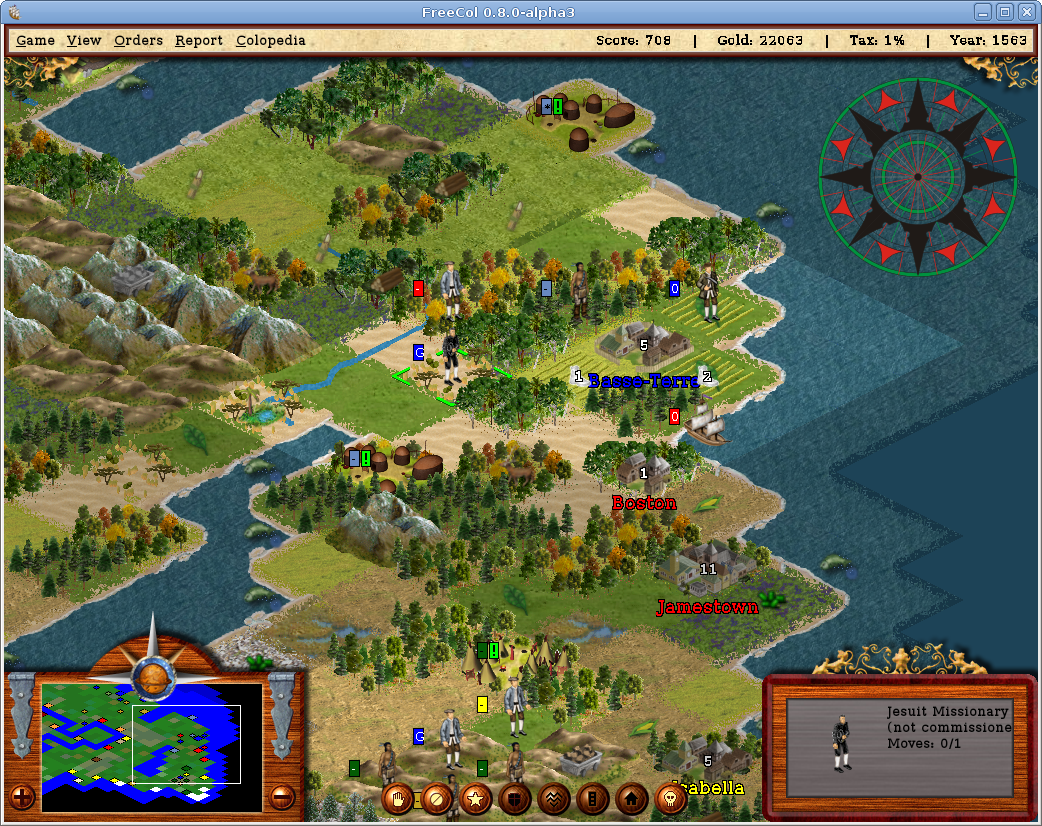
\includegraphics[scale=0.35]{images/main_screen.png}
    \caption{The main screen.\label{main_screen_fig}}
  \end{center}
\end{figure}

The main screen consists of up to six different areas: the menu bar at
the top, the minimap in the lower left corner, the info panel in the
lower right corner, the order buttons between the minimap and the info
panel, the compass rose in the top right corner, and the main map in
the background. The units, colonies, and so forth can be seen on the
main map. They are also represented as coloured dots on the minimap.
The \hyperlink{client options}{preferences menu} allows you to disable
some of these controls if you wish to do so.

\hypertarget{menubar}{\subsection{The Menubar}}

The menubar contains the Game, View, Orders, Report and Colopedia
submenus at the left hand of the screen, as well as a status area at
the right hand of the screen. The status area displays your score, the
amount of gold you possess, your current tax rate and the current
turn.

The \hypertarget{game menu}{Game Menu} allows you to:

\begin{itemize}
\item start a new game
\item open a savegame
\item save the current game
\item change your preferences
\item reconnect to the server
\item chat with another player
\item declare independence
\item end your turn
\item return to the main menu
\item view high scores
\item retire from the game
\item quit the game entirely
\end{itemize}

The \hypertarget{view menu}{View Menu} allows you to:

\begin{itemize}
\item turn the map controls (minimap and info panel) on or off
\item turn the map grid on or off
\item turn borders on or off
\item switch between the unit view and the terrain view
\item switch between full-screen mode and windowed mode
\item display tile names, owners, regions or none of the above
\item change the zoom level of the main map
\item switch to the Europe panel
\item display trade routes
\item center the map on a known settlement
\end{itemize}

The \hypertarget{orders menu}{Orders Menu} enables you to give orders
to the currently selected unit:

\begin{itemize}
\item switch to sentry mode
\item fortify
\item go to a destination you select
\item go to a tile you select
\item execute goto orders
\item assign trade route
\item build or join a colony
\item plow the tile the unit is on (requires 20 tools)
\item build a road on the tile the unit is on (requires 20 tools)
\item load a carrier if possible
\item unload all goods and units on board if possible
\item wait until other units have moved
\item skip this turn
\item switch to a different unit on the same tile
\item clear current orders
\item change the unit's name
\item disband the unit
\end{itemize}

Note that not all orders are available at all times. The build colony
order is only available if the unit is able to build colonies and the
tile it is on will support a colony, for example. The unload order is
only available if the unit is carrying goods. You can unload the goods
anywhere, but if you are not in Europe or in a colony, the goods will
be lost.  You can use this feature to dump unwanted cargo\index{dump
  cargo} in order to avoid the \hyperlink{Cargo Penalty}{cargo
  penalty}.

The \hypertarget{reports menu}{Reports Menu} provides access to
various reports on the current state of your colonies. In these
reports, icons as well as blue text strings link to the places they
refer to. If you click on the name of a colony, for example, the
\hyperlink{colony panel}{Colony Panel} will be opened.

\begin{itemize}
\item The \Report{Religious Advisor} tells you how many crosses your
colonies produce, and how many crosses are required in order to
recruit the next emigrant in Europe.
\item The \Report{Labour Advisor} tells you which types of colonists
have emigrated to the New World or are waiting in Europe. If you can
not remember where you sent your only Expert Ore Miner, for example,
you can use this report to locate him.
\item The \Report{Colony Advisor} tells you which units are present in
each of your colonies, what each colony is producing, which buildings
have already been built, and which building is currently being built.
\item The \Report{Foreign Affairs Advisor} tells you about your
  relations with foreign powers, the number of colonies and units they
  possess, as well as their relative naval and military strength, and
  the amount of gold they possess. As soon as \hyperlink{Jan de
    Witt}{Jan de Witt} has joined the \hyperlink{Continental
    Congress}{Continental Congress}, you are also informed about the
  number of Founding Fathers, the current tax and the current Sons of
  Liberty membership of your opponents.
\item The \Report{Indian Advisor} tells you about your relations with
the various Indian nations, and the number of settlements they
possess.
\item The \Report{Continental Congress Advisor} tells you which
Founding Fathers are already present in the \hyperlink{Continental
Congress}{Continental Congress} and which Founding Father is currently
being elected.
\item The \Report{Military Advisor} informs you of the deployment of
your military units, as well as the strength of the \hyperlink{Royal
Expeditionary Force}{Royal Expeditionary Force}.
\item The \Report{Naval Advisor} informs you of the whereabouts of
your naval units, as well as the strength of the \hyperlink{Royal
Expeditionary Force}{Royal Expeditionary Force}.
\item The \Report{Trade Advisor} details the current market prices of
all goods, the profits before and after taxes you have made, as well
as the amount of goods present in each of your colonies. Colonies that
have already built the \hyperlink{Custom House}{Custom House} are
highlighted, as are all goods that are currently being automatically
exported from these colonies.
\item The \Report{Turn Report} presents a summary of various events
  that have occurred during the current turn. If no such events have
  occurred, the Turn Report will not open.
\item The \Report{Requirements Report} gives an account of how well
certain requirements of your colonies are met. It tells you which
colonies require expert units and where these units can be obtained or
trained, for example. It also tells you which colonies require raw
materials in order to increase their production of manufactured goods,
and which colonies produce a surplus of these materials.
\item The \Report{Exploration Report} provides some information about
  the regions you have discovered and named. If you did not select the
  exploration option, then the report will only show you when you
  discovered the Pacific Ocean, provided you did discover it.
\item The \Report{History Report} contains a short overview of
  important events that took place during the game, such as the first
  meeting with native tribes, the foundation and abandonment of
  colonies, among other things.
\item The \Report{Production Report} provides you with an overview of
  the production of up to four different kinds of goods in your
  colonies, as well as the buildings that produce these goods.
\item The \Report{Education Report} shows you the schoolhouses,
  colleges and universities in your colonies, as well as a list of
  potential teachers and potential students.
\item The menu item ``Show Difficulty Level'' displays the
  \hyperlink{difficulty level}{difficulty level} of the current game.
\item The menu item ``Show Game Options'' displays the \hyperlink{game
  options}{Game Options} of the current game.
\item The menu item ``Show Map Generator Options'' displays the
  \hyperlink{map generator options}{options} that produced the map
  used by the current game.

\end{itemize}

The \hypertarget{colopedia menu}{Colopedia Menu} provides access to
the online game help, which is divided into eight sections:

\begin{itemize}
\item The terrain section contains information on all the different
types of terrain you may encounter in the New World.
\item The bonus resources section lists the special resources of the
  New World. These resources greatly increase the production of
  certain goods. In some cases, tiles can only produce particular
  goods if a resource is present.
\item The goods section gives on overview of all the types of goods in
the game.
\item The unit section provides details on various types of units,
  your own as well native units and units of the Royal Expeditionary
  Force. Skilled units are not included.
\item The skills section lists the various expert units you may
  recruit or train.
\item The buildings section provides information on the various
constructions you may build in your colonies.
\item The Founding Father section can be used to look up information
on the various Founding Fathers you may elect to the Continental
Congress.
\item The nations section tells you which nations are available in the
  game, which national advantage they currently have, and which one
  they have by default.
\item The national advantages section tells you which national
  advantages are available. Some advantages only apply to European
  players, others only to native players.
\end{itemize}


\hypertarget{info panel}{\subsection{The Info Panel}}

If you are in unit view mode (the default), the info panel in the
lower right corner of the screen either shows information about the
currently selected unit, or contains a button to end the current turn
if no unit is selected. If a unit is selected, then the info panel
shows an image of the unit, as well as its name and the moves it has
left. If the unit is a carrier unit, such as a ship or wagon train,
the info panel also shows the units or goods on board of the
carrier. If the unit is a pioneer, the info panel shows the number of
tools the unit carries.

If a unit is displayed, you can click on the info panel in order to
centre the map on this unit.

If you are in terrain view mode, then the info panel displays the
name, owner, defense bonus, movement cost and potential production of
the selected tile. You can switch between view modes by pressing
\verb$Shift-Ctrl-V$, or by using the view menu.


\hypertarget{minimap}{\subsection{The Minimap}}

The minimap in the lower left corner of the screen shows you a more
abstract view of the map than the main map. Different types of terrain
are distinguished by colour, and units and settlements are also
represented by dots in the colour of the nation that owns them. You
can use the minimap to navigate around the map quickly.  Either click
on the minimap to center the view on a certain point, or drag the
white frame around. Zoom buttons to the left and to the right of the
minimap allow you to zoom into and out of the view.


\hypertarget{unit buttons}{\subsection{The Unit Buttons}}

The unit buttons displayed between the minimap and the info panel
allow you to give order to your units. Note that not all buttons are
always active. A ship can not plow a tile, for example, so the plow
button is never active if the selected unit is a ship. The eight
buttons have the following functions:

\begin{itemize}
\item wait
\item skip turn
\item fortify
\item clear forest / plow tile (requires 20 tools)
\item build road (requires 20 tools)
\item build colony
\item disband unit
\end{itemize}

All these actions are also available from the \hyperlink{orders
menu}{Orders Menu} of the menu bar, and as \hyperlink{keyboard
shortcuts}{keyboard shortcuts}.


\hypertarget{compass rose}{\subsection{The Compass Rose}}

The compass rose can be displayed in the top right corner and allows
you to give your units movement orders by clicking on the corresponding
direction. It is primarily intended for users who do not wish to (or
are unable to) use the keyboard shortcuts.


\hypertarget{main map}{\subsection{The Main Map}}

The main map shows you the New World in greater detail. You can see
the different types of terrain, forested and otherwise, hills,
mountains, rivers, and, of course, the various units and settlements
of the native and European players.  Sometimes units will be all
grey---this shows the position of the unit when you could last see
that tile, but does not guarantee that the unit is still there.  Left
click on a tile in order to center the main map, or on a unit in order
to select it (a \hyperlink{display options}{display option} allows you
to decide whether the map should always centre on the selected unit,
or not).

Your colonies as well as those of your opponents are displayed on the
map. You can see their names as well as their sizes, which are
displayed as a number and also influence the image used to represent
them. The color of the colony's name is always the color of its owner,
but the color of the colony size indicates whether any production
bonuses or penalties apply (at normal difficulty):

\vskip5mm

\begin{tabular}{l r l}
Colour&Bonus/Penalty&Requirements\\
\hline
Red    & -2 & more than eight tories\\
Orange & -1 & four to seven tories\\
White  &  0 & less than four tories and less than 50\% SoL\\
Green  & +1 & 50\% SoL or more\\
Blue   & +2 & 100\% SoL\\
\end{tabular}

\vskip5mm

Left click on a colony in order to open the \hyperlink{colony
  panel}{colony panel}. If there is an active unit outside of the
colony on the same tile, then a single left click will select the unit
instead. In this case, a double click will still open the colony
panel.

Right clicking on an empty tile, will either display some information
on that tile if no unit is selected, or open a pop-up menu that
additionally allows you to send the selected unit to this tile. If the
tile contains some of your units, the menu will also enable you to
select each of these units. If the tile contains a native settlement,
the menu will also provide you with an item that will bring up some
information on that settlement. If the tile contains one of your own
colonies, the menu will also allow you to open the \hyperlink{colony
panel}{colony panel}.

You can also activate the map scroll by moving the cursor towards the
edges of the main map. Scrolling with the minimap is faster, however.

If a unit is selected, further information about that unit is
displayed in the \hyperlink{info panel}{info panel}, and you can move
the unit\index{unit movement} using the numeric keypad or the
\hyperlink{compass rose}{compass rose}. If you select a unit with the
left mouse button and drag the mouse, the main map will display the
best path from the unit's current position to the tile the mouse is
hovering over.

The tiles the path consists of will be marked with boots if the unit
is on foot, with horseshoes if the unit is mounted, with wheels if the
unit is a wagon train, or with sextants if the unit is a naval
unit. Full-colour symbols mark tiles that can be reached in the same
turn, whereas shaded symbols mark tiles that can be reached only in
subsequent turns. A number indicates how many turns later the unit
will arrive on this tile. You can see this on the \hyperlink{main
  screen}{main screen}.


  \begin{center}
    
\includegraphics{images/path-foot.png}
    
\includegraphics{images/path-horse.png}
    
\includegraphics{images/path-wagon.png}
    
\includegraphics{images/path-naval.png}
  \end{center}


Once you release the mouse button, the selected unit will begin to
follow this path. It will awake once it has arrived at its destination
or if it can no longer follow the path (if a unit belonging to a
different player is in the way, for instance). You can also press the
middle mouse button, or both mouse buttons if your mouse only has two
buttons, in order to give the selected unit a movement order.

In the original Colonization game, a unit always used up all movement
points when entering a colony. In FreeCol, this is not the case---a
unit can enter a colony just like any other tile. If the unit is
placed in a building, or on a colony tile, or if a carrier is loaded
or unloaded, however, it will lose all its movement points.

Units are marked with small coloured shields, which may or may not
display a letter. The background colour indicates the nation this unit
belongs to. The Dutch units, for example, are usually marked with
orange shields. The letter indicates the current state of the unit:

\pagebreak[2]
\begin{itemize}
\item\verb$-$: the unit is active (no orders).
\item\verb$F$: the unit is fortified.
\item\verb$G$: the unit is going somewhere.
\item\verb$P$: the unit is plowing a tile.
\item\verb$R$: the unit is building a road.
\item\verb$S$: the unit is a sentry (waiting for transport).
\item\verb$T$: the unit is following a trade route.
\item\verb$W$: the unit is waiting for orders (skipped).
\item\verb$0$: the unit has no moves left.
\item\verb$#$: the unit's state is unknown (some enemy units).
\end{itemize}

If the unit is a foreign naval unit, the shield will display a number
instead. This is the number of holds this unit is using.

Indian Settlements display at least two shields: The colour of the
first shield indicates the nation this settlement belongs to. A $*$ on
this shield indicates that this settlement is the nation's capital, a
$-$ that it is not. The second shield, which bears an exclamation mark
($!$) if you have visited the settlement, and a question mark ($?$) if
you have not, indicates the current relations between the nation and
your colonists. Its background may be green, blue, yellow, orange or
red, depending on whether your relations are good, mediocre or bad.

A Settlement with a European mission displays a third shield bearing a
cross on a black or grey background. The colour of the cross indicates
the European nation that established the mission. The background of
the shield is black if the mission was established by a
\hyperlink{Jesuit Missionary}{Jesuit Missionary}, and grey otherwise.

The preferences menu allows you to select ``modern'' colony labels
instead of these ``classic'' labels. The modern labels display the
same information, but in a slightly different way.

The order buttons represent some of the orders you can give to your
units. You can move your mouse over the buttons to see their
respective orders. If a unit is unable to perform a certain action,
the corresponding order button will be disabled. The orders are also
available from the \hyperlink{orders menu}{Orders Menu}, and you can
use the following \hypertarget{keyboard shortcuts}{keyboard shortcuts}:

\pagebreak[2]
\begin{itemize}
\item\verb$a$: assign a trade route.
\item\verb$b$: build a colony, or join an existing colony.
\item\verb$c$: clear forest (requires 20 tools)
\item\verb$d$: disband the active unit.
\item\verb$e$: show the Europe panel.
\item\verb$f$: fortify.
\item\verb$g$: go to some destination tile.
\item\verb$h$: go to a settlement (or Europe if a ship).
\item\verb$l$: load (fill up all holds already in use).
\item\verb$n$: rename the unit.
\item\verb$o$: execute goto orders immediately.
\item\verb$p$: plow the current tile (requires 20 tools).
\item\verb$r$: build a road on the current tile (requires 20 tools).
\item\verb$s$: be a sentry (wait for something to happen).
\item\verb$t$: show trade routes.
\item\verb$u$: unload or dump cargo.
\item\verb$w$: wait for another unit to move.
\item\verb$z$: clear orders.
\item\verb$tab$: switch to next unit on tile, or to colony screen.
\item\verb$space$: skip for this turn.
\item\verb$enter$: end the turn.
\item\verb$plus$ or \verb$equals$: zoom in.
\item\verb$minus$ or \verb$underscore$: zoom out.
\item\verb$ctrl-c$: center on the currently selected unit.
\item\verb$ctrl-d$: display tile names.
\item\verb$ctrl-f$: find a colony.
\item\verb$ctrl-g$: display grid.
\item\verb$ctrl-m$: show/hide the map controls.
\item\verb$ctrl-n$: new game.
\item\verb$ctrl-o$: open a game.
\item\verb$ctrl-q$: quit the game.
\item\verb$ctrl-r$: reconnect.
\item\verb$ctrl-s$: save a game.
\item\verb$ctrl-t$: show the chat panel.
\end{itemize}

You can customize these settings in the preferences dialog.


\hypertarget{europe panel}{\section{The Europe Panel}}

The figure \ref{europe_panel_fig} represents the Europe panel.
\begin{figure}[htb]
  \begin{center}
    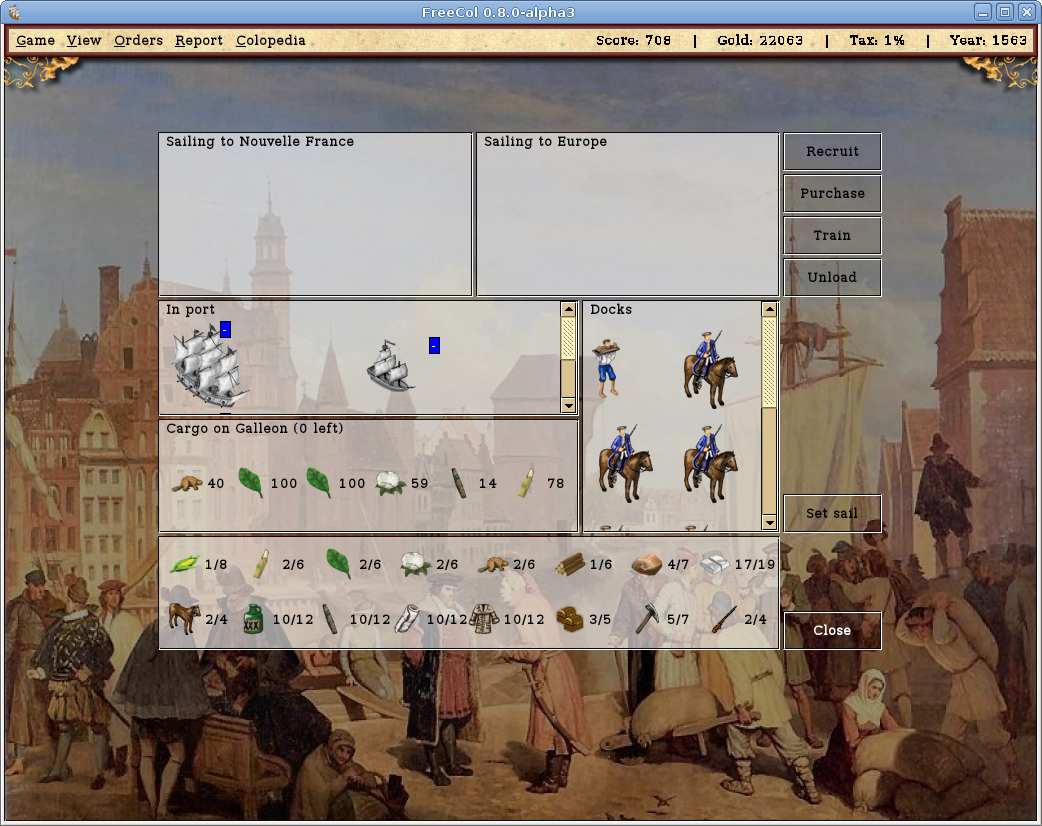
\includegraphics[scale=0.35]{images/europe_panel.png}
    \caption{The Europe Panel\label{europe_panel_fig}}
  \end{center}
\end{figure}

In this panel, you can control the ships sailing between America and
Europe, as well as the ships currently docked in Europe. You can also
buy goods, recruit, purchase and train units. Units recruited,
purchased or trained are visible in the Docks Area in the Europe
panel.

If a ship has set sail for Europe or America, you can change its
direction by dragging it from the Going to America box to the Going
to Europe box (or vice versa).

If a ship has docked at the European port you can drag and drop units
between the Docks and Cargo panel. You drag and drop goods between the
Cargo panel and the Market panel. If you want to buy or sell less than
100 units of goods, press the shift key while dragging. This will
allow you to specify how many units you wish to transfer. If you press
the ``Unload'' button, all goods will be unloaded.

If any of the goods are displayed in grey, this means they are being
boycotted by the Crown because you refused a tax raise. You must pay
your tax arrears before you can trade these goods. You can do this by
dragging the goods as usual, in which case you will be given the
chance to pay your tax arrears (provided you have enough money). A
small area at the top right of the screen will keep track of how much
money you made or spent and how much taxes you paid.

From time to time, new colonists eager to join you in the New World
will appear on the European Docks. If you are unwilling to wait, you
can also recruit new colonists by paying for their journey to the New
World. Alternatively, you can train expert units at the Royal
University. Paying for their education is expensive, however, and not
all types of experts are available in Europe.

Units present in Europe can also be armed, mounted, equipped with
tools or blessed as missionaries in Europe. In order to select one of
these actions, you need to right click on the unit. Note that you will
have to pay for the arms, horses or tools required to equip your
units. Blessing a missionary, however, is free.

In order to send a ship back to the New World, you must drag it to the
Going to America section of the Europe panel, or press the ``Set
sail'' button.


\hypertarget{colony panel}{\section{The Colony panel}}

The figure \ref{colony_panel_fig} represents the Colony panel.
\begin{figure}[htb]
  \begin{center}
    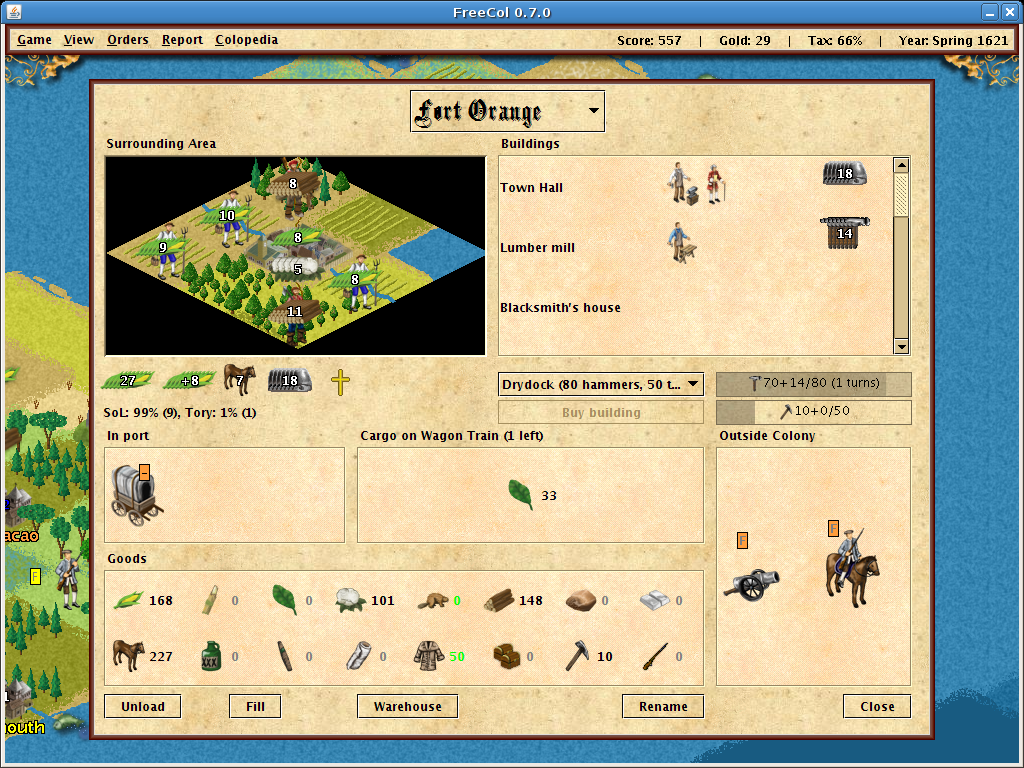
\includegraphics[scale=0.35]{images/colony_panel.png}
    \caption{The Colony Panel\label{colony_panel_fig}}
  \end{center}
\end{figure}

To view a colony's panel, left click on it from the main screen. In
this panel, colonists can be assigned to cultivate tiles surrounding
the colony, to work in buildings, defend the colony against attackers
or wait outside of the colony.

The select box at the top left of the panel displaying the name of the
colony can be used to select a different colony. You can also use the
``left'' and ``right'' keys to ``scroll'' through your colonies. Next
to the colony's name, the production panel shows all the goods your
colony is producing.

Below colony name, you can see the area surrounding the colony to the
left and a scroll pane displaying the buildings of the colony to the
right. You can drag and drop a unit on a tile or a building. Buildings
only ever produce a single type of goods. The tiles surrounding the
colony can produce several kinds of goods, however. If the unit is not
producing the right kind of goods, you can right click on the unit to
select a different kind of work. If a tile has a red border, then it
can not be used---it is either assigned to another colony or
settlement, or is occupied by a hostile unit, or is a water tile which
can not be used until you have built \hyperlink{Dock}{docks}.  Note
that if you drag a unit onto a tile owned by the natives you may be
offered the chance to purchase the land.

Below the surrounding area, you can see the population panel, which
displays the size of your colony, the number and percentage of
colonists that support independence, the number and percentage of
colonists that support the crown, as well as the current production
bonus.

Below the status panel, the port panel shows you any ships or wagon
trains in the colony. If there is at least one unit present, the cargo
panel below the port panel shows you the cargo of the selected carrier
(if any).

On the right hand side of the panel, you can see the buildings panel,
which displays an image for every building in the colony, as well as
the building or unit currently being built. You can see the units
working in a building, as well as its production. If you let the mouse
hover over a building, you can see a slightly larger and more detailed
view. You can click on any building in order to open the build queue
dialog, which enables you to create a list of units and buildings to
build.

Below the buildings panel, the outside colony panel shows you which
colonists are present on the same tile, but are not working inside the
colony. Any units shown here are able to defend the colony against
attacks.

Below this panels, you can see the colony's warehouse area. You can
drag and drop goods from the warehouse to the cargo panel and vice
versa in order to load and unload your ships or wagon trains. Press
the shift key while selecting goods if you do not wish to select all
the goods present, or less than one hundred units.

The \hyperlink{Warehouse}{Warehouse} can only hold a certain amount of
goods of each type. Its initial capacity is limited to 100 units of
each type of goods, but it can be increased to 300 by building two
\hyperlink{Warehouse Expansion}{Warehouse Expansions}. If the current
limit of the warehouse is exceeded, the number of goods is printed in
red. If you do not store the excess units elsewhere, they will be lost
at the end of the turn.

If you have already built a \hyperlink{Custom House}{Custom House} in
the colony, you can export goods to Europe automatically. Goods marked
to be exported are printed in green. Open the warehouse dialog (see
below) in order to change export settings.

At the bottom of the Colony Screen, you will see a row of buttons, not
all of which are always active. These buttons will allow you to

\begin{itemize}
\item Unload the active ship or wagon train
\item Fill up all partially filled holds of the active ship or
wagon train
\item Open the warehouse dialog in order to change the export and
  warning levels for all types of goods (see \hyperlink{The Warehouse
    Dialog}{below})
\item Select which buildings or units to build (see \hyperlink{The
  Build Queue Panel}{below}).
\item Close the dialog
\end{itemize}

You can drag and drop colonists to and from buildings, tiles
surrounding the colony, ships and the area outside of the colony. You
can also use the right click menu of any unit to assign it to a work
place, equip it, or place it outside of the colony (unless it already
is outside of the colony).



\hypertarget{The Warehouse Dialog}{\subsection{The Warehouse Dialog}}

The warehouse dialog allows you to set the warning levels for all
types of goods. If you have turned on the warnings about goods levels,
you will receive a warning if the number of goods drops below the
lower level or rises above the higher level. In a warehouse with a
capacity of 100 units of each type of goods, the lower level is set to
10 and the higher level is set to 90 by default.

The export level allows you to specify how many goods should be kept
in reserve if goods are automatically exported from this colony,
either through the \hyperlink{Custom House}{Custom House}, or by a
carrier following a \hyperlink{Trade Routes}{Trade Route}. A checkbox
indicates whether this type of goods should be exported through the
Custom House or not. If you have not yet built a Custom House in this
colony, the checkbox is disabled.


\hypertarget{The Build Queue Panel}{\subsection{The Build Queue Panel}}

Clicking on a building (not one of the units working in the building)
opens the build queue panel, which allows you to select which items
the colony should build. The panel consists of three sub-panels, the
unit panel on the left, the buildings panel on the right and the build
queue in the centre. You can drag and drop items from the unit panel
and the buildings panel to the build queue and back. You can also
double-click an item in the unit panel or the building panel to add it
to the build queue, and you can double-click an item in the build
queue to remove it. Right-click an item to see its entry in the
Colopedia.

The panel contains a checkbox that switches between the compact view,
which shows only the names of the buildable items, and the icon view,
which also shows the goods required to build each item. Another
checkbox allows you to see items that the colony can not build at this
time because it lacks the necessary population, or because some other
requirement has not yet been met. You can also add these items, which
are marked with a small lock icon, to the build queue, but not as the
head of the queue.

The ``buy building'' button allows you to buy the building at the top
of the build queue, provided that you have enough gold.


\hypertarget{customization}{\section{Customization}}

The FreeCol user interface can be customized to a certain degree. In
the directory where FreeCol is installed, you will find a
sub-directory called {\tt data}, which contains configuration files
and multimedia assets. These include the images used to represent
units, goods, buildings and various other objects that appear in the
game, sounds to play when certain events occur and so forth. You can
replace them if you wish.

The sub-directory {\tt data/base/} contains assets that are used for
the user interface in general, independent of the rules used for a
particular game. The sub-directory {\tt
  data/\-base/\-resources/\-fonts} contains several fonts\index{fonts}
that are distributed with FreeCol, including the file {\tt
  ShadowedBlack.ttf}, which contains the black letter font used to
display headlines and the titles of panels. The file {\tt
  data/\-base/\-resources.properties} allows you to configure how the
assets are used.

The line

\begin{quote}
{\tt NormalFont=urn:font:Serif-PLAIN-13}
\end{quote}

for example, selects the font called ``Serif'' with font style
``plain'' and font size 13. Instead of ``Serif'', you could use any
other font that is known to the Java Virtual Machine of your
system. In general, this includes all fonts installed by the operating
system (rather than individual applications).

Please note that FreeCol uses a Uniform Resource Identifier (URI) to
identify the font. For this reason, you must obey the usual quoting
rules. In particular, you must use the string {\tt \%20} instead of a
space character in the font name.

In order to use a TrueType font that is not available to the JVM, you
must copy it to the fonts directory mentioned above and add it to the
configuration file by adding a line like this:

\begin{quote}
{\tt MyFavouriteFont=resources/fonts/Chancery.ttf}
\end{quote}

Then you could say:

\begin{quote}
{\tt NormalFont=urn:font:Black\%20Chancery-PLAIN-13}
\end{quote}

Instead of {\tt MyFavouriteFont}, you can any key you like, as long as
it is not being used for anything else. This line will add your font
to the list of fonts known to the JVM, and you can then use its name,
which is, however, likely to differ from the file name. The file {\tt
  Chancery.ttf}, for example, contains a font called ``Black Chancery''.


\hypertarget{The New World}{\chapter{The New World}}

At the beginning of the game, you will start with a naval vessel and
two colonists. Your first task will be to discover the New World,
which should lie due West, although sailing North West or South West
may prove quicker. As soon as you have discovered land, you can
establish your colonies and produce goods to send home to Europe.

\hypertarget{Terrain Types}{\section{Terrain Types}}

There are many different types of terrain in the New World, each with
its own peculiar advantages. At the beginning of the game you will
probably arrive at a \Terrain{High Seas} tile (or at the edge of the
map). High Seas tiles (and the map edge) allow you to sail between
Europe and the New World. As you approach land, the High Seas will be
replaced by \Terrain{Ocean} tiles, which produce
\hyperlink{Fish}{Fish}.

In the New World, you will also discover \Terrain{Plains}, which
produce a great deal of Grain, a lesser amount of Cotton, and some
Ore; \Terrain{Grassland}, on which Grain and Tobacco can be
cultivated; \Terrain{Prairie}, which are suitable for growing Grain
and Cotton; \Terrain{Savannah}, which produces Grain and Sugar;
\Terrain{Marsh}, where Grain can be cultivated and some Ore can be
mined; \Terrain{Swamp}, which yields some Grain, and small amounts of
Sugar, Tobacco and Ore; \Terrain{Desert}, which produce some Food,
Cotton and Ore; as well as \Terrain{Tundra}, where Grain can be grown,
and some Ore can be mined.

Large parts of the New World are covered in forests, all of which
yield varying amounts of Grain, Lumber and Furs. The \Terrain{Boreal
Forest} also produces Ore, the \Terrain{Mixed Forest} Cotton, the
\Terrain{Conifer Forest} Tobacco, the \Terrain{Tropical Forest} Sugar,
the \Terrain{Rain Forest} produces small amounts of Ore, Sugar and
Tobacco, the \Terrain{Wetland Forest} and the \Terrain{Scrub Forest}
yield some Ore, and the \Terrain{Broadleaf Forest} Cotton.

The \Terrain{Hills} produce a small amount of Grain, and can be mined
for Ore and a lesser amount of Silver. The \Terrain{Mountains} are
unsuitable for agriculture, but yield some Ore and Silver.
\Terrain{Arctic} tiles are the least useful type of terrain, as they
produce nothing at all. Terrain types that produce no Grain, such as
the Mountains and Arctic types, can not support colonies.

Clearing or plowing a tile, and building a road require spending 20
tools. Therefore, these actions can only be carried out by units
carrying at least 20 tools. You can equip your units in your colonies
or in Europe.

\hypertarget{Goods}{\section{Goods}}

The New World produces many goods, which can be traded in Europe. In
order to this, you must use your ships to transport them to your
\hyperlink{Home Port}{Home Port}. As soon as the ship arrives in
Europe, you can sell the goods, and buy others, in the
\hyperlink{europe panel}{Europe Panel}. Later in the game, after you
have built \hyperlink{Custom House}{Custom Houses}, goods can be
exported automatically. Until then, you can partially automate this
process by establishing \hyperlink{Trade Routes}{Trade Routes}.

Exporting these goods to Europe will be one of your most important
sources of income. At the beginning of the game, you will probably
want to export raw materials, such as \textbf{Sugar} and
\textbf{Tobacco}, but as prices drop, you should concentrate on luxury
products, such as \textbf{Rum} and \textbf{Cigars}, which command
higher prices.

\Goods{Food} is the single most important good, since all your
colonists consume two units of food each turn. If this demand can not
be met, some of your colonists will starve to death.  On the other
hand, a colony that has accumulated 200 units of food will produce a
new \hyperlink{Free Colonist}{Free Colonist}. Unfortunately, buying
food in Europe is always expensive, and colonial foodstuffs fetch only
poor prices.

Food is produced from two basic food stuffs, \Goods{Grain}, which can
be cultivated on nearly all land tiles, and \Goods{Fish}, which is
produced by \hyperlink{Ocean}{ocean} and lake tiles. To harvest the
bounty of the sea, you will need a \hyperlink{Dock}{Dock}, however.

\Goods{Horses} are special in several ways. Horses will survive by
grazing in your colonies' \hyperlink{Pasture}{Pastures}, but in order
to reproduce they require grain, and there have to be at least two of
them. Horses live in herds, and each herd produces no more than two
new horses per turn. In the Pasture, a herd consists of fifty horses,
but in the \hyperlink{Stables}{Stables}, a herd consists of only
twenty-five horses, effectively doubling the number of horses you can
breed per turn (provided you have enough food).

The number of horses you can breed is further limited by the fact that
horses feed only on grain and not on fish. And Pastures and Stables
consume no more than half the food surplus available. In other words,
you can not breed more horses by filling your colonies' warehouses
with grain.

Four raw materials are typical for the New World. They will initially
generate a good income, but prices will inevitably drop. These goods
are \Goods{Sugar}, which is best cultivated on
\hyperlink{Savannah}{Savannah} tiles, \Goods{Tobacco}, best cultivated
on \hyperlink{Grassland}{Grassland}, \Goods{Cotton}, which is most
abundant on \hyperlink{Prairie}{Prairie} tiles, and \Goods{Furs},
which are available on all forested tiles, but most abundantly on
\hyperlink{Boreal Forest}{Boreal Forest} and \hyperlink{Mixed
Forest}{Mixed Forest} tiles.

These four materials can be used to produce corresponding luxury
goods, which will fetch much higher prices in Europe. In a
\hyperlink{Distiller's House}{distillery}, \Goods{Rum} is produced
from Sugar. Tobacco is used to make \Goods{Cigars} in the
\hyperlink{Tobacconist's House}{Tobacconist's House}. The Weaver
weaves \Goods{Cloth} from Cotton in his \hyperlink{Weaver's
House}{house}, and the Fur Trader turns Furs into \Goods{Coats} in his
\hyperlink{Fur Trader's House}{house}.

Initially, the resource which fetches the highest prices in Europe is
\Goods{Silver}, which can be mined in the
\hyperlink{Mountains}{Mountains}. Small amounts of silver can also be
produced on \hyperlink{Swamp}{Swamp} and \hyperlink{Marsh}{Marsh}
tiles with a minerals resource.

As prices drop, Silver will become less and less useful, however. On
the other hand, Hills and Mountains also produce \Goods{Ore}, which is
not in great demand in Europe, but which can be refined to produce
\Goods{Tools} in the \hyperlink{Blacksmith's House}{Blacksmith's
  House}. Tools are required for clearing forests and plowing fields,
as well as for constructing advanced buildings and units. Furthermore,
\Goods{Muskets} can be produced from Tools in the
\hyperlink{Armory}{Armory}.

\Goods{Lumber} also fetches poor prices in Europe, but can be used to
produce \Goods{Hammers} in the \hyperlink{Carpenter's
House}{Carpenter's House}. Hammers are required for constructing all
buildings, as well as \hyperlink{Naval Units}{naval units} and
\hyperlink{Wagon Train}{Wagon Trains}. Hammers are ``abstract'' goods
that can neither be transported nor traded. They represent the work
required to finish a building rather than some tangible material.

The two other ``abstract'' goods are \Goods{Liberty Bells}, which are
produced in the \hyperlink{Town Hall}{Town Hall}, and \Goods{Crosses},
which are generated by the \hyperlink{Church}{Church}. They represent
the concepts of liberty and of religious freedom. Liberty Bells
produce \hyperlink{Liberty}{liberty points}, which are needed to
convince your colonists of your policies, and to elect
\hyperlink{Founding Fathers}{Founding Fathers} to the
\hyperlink{Continental Congress}{Continental Congress}. Crosses
generate \hyperlink{Immigration}{immigration points}, which are needed
to attract further immigrants in Europe.

\Goods{Trade Goods}, on the other hand, can be transported and traded,
but they can not be produced in your colonies. They are only available
in Europe and are useful for trading with native settlements, which
generally demand Trade Goods.


\hypertarget{Trade Routes}{\subsection{Trade Routes}}

The \hyperlink{orders menu}{orders menu} allows you to assign a Trade
Route to a ship or wagon train. If you select this order, the trade
route dialog, which enables you to select a trade route or create a
new trade route, will open. If you have not created a trade route, you
must use the edit trade route dialog to do so first.

A trade route consists of two or more stops, which may either be the
\hyperlink{Home Port}{Home Port}, or one of your colonies. Select a
destination from the select box and press the \texttt{add new stop}
button. If you select the special destination \texttt{all colonies},
then your Home Port and all your colonies will be added to the list of
stops.

If you have selected a destination, you can drag and drop goods from
the goods panel to the cargo panel. These are the goods your ship or
wagon train should have on board when leaving this stop. If the ship
or wagon train arrives at the destination with other goods on board,
these goods will be unloaded.

Note that the ships and wagon trains will take the capacity and
settings of the warehouses in your colonies into account. They will
not unload cargo that would be wasted and they will only load goods
that should not be kept in reserve. This means that they may wait
for a long time until a sufficient number of goods becomes available.

As soon as a ship or wagon train reaches the last destination of the
trade route, it will continue at the first destination.

The behaviour of trade routes can sometimes be confusing.  To see
exactly what each unit with a trade route is doing, enable the
\texttt{Goods Movement} message type, but beware that there can be
many messages of this type.

\hypertarget{Resources}{\section{Special Resources}}

Some types of terrain can also have special resources, which increase
the production of a particular type of goods. Most of these resources
look just like the goods they will produce. These tiles are
particularly valuable.


\hypertarget{Native Settlements}{\section{Native Settlements}}

The New World is by no means an uninhabited country. Various tribes of
Indians already live there, and make use of the land. When your
colonists arrive, you will have to decide whether you will attempt to
peacefully coexist with the natives, or to wipe them out. The
\hyperlink{France}{French} player has the advantage of generating only
half the alarm among the natives. The \hyperlink{Spain}{Spanish}
player has the advantage of greater military efficiency against the
natives. Your choice of \hyperlink{Home Country}{Home Country} may
influence your strategy---or vice versa.

Small Native Settlements use the tile they are built on and all the
adjacent tiles, just like your \hyperlink{Colonies}{Colonies} do, and
possibly more nearby tiles. Large Native Settlements also use tiles
that are two moves away, and possibly more. Your colonists can not use
tiles that are already used by natives. If they attempt to do so, the
natives will demand some gold for the land. You must then decide
whether to pay their price, take the land away from the by force, or
to leave the land alone.  Naturally, the natives will not be pleased
if you take the land away from them. As soon as \hyperlink{Peter
  Minuit}{Peter Minuit} has joined the \hyperlink{Continental
  Congress}{Continental Congress}, however, the natives no longer
demand payment for their land nor become immediately displeased if it
is taken.

A special case exists for the center tile of the colonies you found.
In the ``classic'' ruleset and/or by default in when playing under the
``Very Easy'' difficulty level the center tile does not have to be
paid for.  ``Easy'' difficulty restricts this to only apply to a
single colony, ``Normal'' to a single colony and requires the tribe
you are stealing land to have not been contacted, and other levels
require payment as usual.

Colonies and armed units near their settlements will alarm the natives
and poison your relations. If the natives are happy, they will come to
your colonies offering gifts. If they are unhappy, they will come and
make demands instead. If they get really angry, they may attack your
units or colonies. After a few turns, however, they will usually calm
down again.

Some types of units may enter Native Settlements. Units that carry
goods, such as \hyperlink{Wagon Train}{Wagon Trains} and
\hyperlink{Naval Units}{Ships}, can enter the settlements and trade
with them. Trade always improves your relations with the natives. If
you offer your goods as a gift, this will improve your relations even
more.

\hyperlink{Scout}{Scouts} can either ask to speak with the chief of
the tribe, or demand tribute, which is obviously not good for your
relations with the natives. If your scout speaks with the chief, you
will learn which skill this settlement teaches and which goods the
natives would prefer to acquire. Furthermore, the chief may offer you
some gold, or tell you about nearby lands. If your Scout is not a
\hyperlink{Seasoned Scout}{Seasoned Scout} already, he may become so.

\hyperlink{Free Colonist}{Free Colonists} and \hyperlink{Indentured
Servant}{Indentured Servants} may enter a settlement in order to learn
the skills of the natives.

\hyperlink{Missionary}{Missionaries}, which may be either
\hyperlink{Jesuit Missionary}{Jesuit Missionaries} or ordinary
colonists blessed as missionaries in the \hyperlink{Home Port}{Home
  Port} or any colony with a \hyperlink{Church}{Church}, are able to
establish a \Concept{Mission} or to incite the natives against another
European nation. If a Jesuit Missionary, or an ordinary colonist
blessed as a missionary is equipped with tools, muskets or horses, he
loses his missionary status and is no longer able to establish a
mission.

The presence of a Mission will reduce tension between the natives and
your colonists. In time, some of the natives may also convert and join
your colonies as \hyperlink{Indian Convert}{Indian Converts}. If the
settlement already contains the mission of another European country,
your missionary may denounce the teachings of that mission as a
heresy. If he is successful, the natives will burn down the old
mission and your missionary establishes a new one.

Note that the missionary will always remain in the settlement. He is
effectively lost to you.


\hypertarget{Lost City Rumours}{\section{Lost City Rumours}}

In the New World, there are also rumours about \Concept{Lost Cities},
such as El Dorado, or C{\'\i}bola. The natives do not explore these
sites, but your colonists can and, in fact, must do so if they enter a
tile with a Lost City Rumour. It is not possible to farm a tile with a
Lost City Rumour on it.

Mostly, the rumour proves to be nothing but a rumour. Occasionally,
you might disturb the burial grounds of a native tribe, which will
cause the tribe to declare war on you. It is also possible that your
expedition simply vanishes without a trace.

On the other hand, you might also discover a small tribe and a few
trinkets. Your colonist might become a \hyperlink{Seasoned
  Scout}{Seasoned Scout} if he has no other skill, you might discover
the sole survivor of a lost colony, or even one of the Seven Cities of
Gold, and a \hyperlink{Treasure Train}{Treasure Train}.

Possibly the best outcome is the discovery of the \Concept{Fountain of
Youth}, which will cause numerous colonists to appear on the docks in
your \hyperlink{Home Port}{Home Port}.

As soon as \hyperlink{Hernando de Soto}{Hernando de Soto} has joined
the \hyperlink{Continental Congress}{Continental Congress}, Lost City
Rumours always yield positive results.


\hypertarget{Exploration}{\section{Exploration}}

The original Colonization game awarded exploration points only for the
discovery of the Pacific Ocean. This is also the default behaviour for
FreeCol. However, you may choose to play with exploration points, in
which case you will be awarded exploration points for the discovery of
a new region of the New World.

A region may be either a large area of land, a mountain range, or a
river valley. If you discover a region, you will be asked to name it,
and you will be awarded a number of exploration points depending on
the size of the region discovered.


\hypertarget{Colonies}{\chapter{Colonies}}

\hypertarget{Picking a suitable site}{\section{Picking a suitable site}}

Your colonies are your most important assets in the new world.
Therefore, it is very important to build them in the right
place. There are several aspects to consider:

\hypertarget{The colony tile}{\subsection{The colony tile}}

The tile your colony is built on is special in several ways. It is the
only tile that produces more than one type of goods at the same time
and neither requires nor allows the presence of a colonist to do
so. On the other hand, you can not choose which types of goods to
produce. The colony tile will always produce some kind of food as its
primary product, and some raw material other than lumber or silver as
its secondary product. The production of food can be increased by
plowing the colony tile, but the secondary production will not benefit
from artificial tile improvements such as fields and roads. It will,
however, benefit from natural tile improvements such as rivers and
resources.

Some terrain types are more suitable for establishing a colony than
others. Colonies can not be built on Arctic tiles, nor on Mountains,
because these terrain types produce no Grain. Hills and Deserts are
less suitable than other tiles because they produce less food, which
is very important in the long run. Tiles with forest generally produce
less food than tiles without, but \hyperlink{Pioneer}{Pioneers} are
able to cut down the forest and plow the tile, which will increase
food production. The presence of a river will also increase food
production.

The \hyperlink{Hills}{Hills} produce a small amount of Grain, and can
be mined for Ore and a lesser amount of Silver. The
\hyperlink{Mountains}{Mountains} are unsuitable for agriculture, but
yield some Ore and Silver. \hyperlink{Arctic}{Arctic} tiles are the
least useful type of terrain, as they produce nothing at all. Terrain
types that produce no Grain, such as the Mountains and Arctic types,
can not support colonies.

The New World is also irrigated by minor and major rivers. The
production of most types of \hyperlink{Goods}{Goods} is increased by
the presence of rivers as well as roads, which your
\hyperlink{Pioneer}{Pioneers} can build. All terrain types which
produce Grain (except the Hills) can also be plowed by your Pioneers
in order increase grain production. If the tile is forested, you must
first clear the forest and transform the tile into open land:

\vskip5mm
\begin{tabular}{l @{\hskip5mm$\rightarrow$\hskip5mm} l}
Forested&Cleared\\
\hline
Boreal Forest & Tundra\\
Mixed Forest & Plains\\
Conifer Forest & Grassland\\
Tropical Forest & Savannah\\
Wetland Forest & Marsh\\
Rain Forest & Swamp\\
Scrub Forest & Desert\\
Broadleaf Forest & Prairie\\
\end{tabular}
\vskip5mm


\hypertarget{The adjacent tiles}{\subsection{The adjacent tiles}}

In the early stages of the game, you will need to generate cash by
selling products from the New World in your Home Port. Thus, many of
your early colonies should probably be situated next to bonus tiles,
which greatly increase production. Rivers also increase production,
though not as much as a bonus resource. On the other hand, they
increase the production of many different kinds of goods, unlike a
bonus resource.

In order to improve your colony, you will have to construct various
buildings. This will require large amounts of lumber. For this reason,
you should make sure that at least one tile adjacent to your colony
site can produce sufficient amounts of lumber. You will also need
tools to construct advanced buildings. Therefore, it is an advantage
if the colony can also produce ore, which can be refined to produce
tools. However, ore is not as important as lumber.

Some of the tiles may be owned by other European powers, or claimed by
Indians. Building a colony too close to other settlements is not a
good idea, unless you plan to conquer or destroy these settlements.
Keeping your own colonies close together is a good strategy, however,
as long as you avoid sharing tiles between several colonies as far as
possible.


\hypertarget{Reforestation}{\subsection{Reforestation}}

You can order your pioneers to cut down forests by plowing a tile.
This will increase the food produced on these tiles, and the lumber
will be delivered to your colonies. Under the usual rules, you can not
plant new forests later, however. Once cleared, a tile will never
produce lumber again. The ``Plant forest'' mod distributed with
FreeCol corrects this issue, however.


\hypertarget{Government Efficiency}{\subsection{Government Efficiency}}

The efficiency of the local governments of your colonies depends on
the colonists' support for the \hyperlink{Sons of Liberty}{Sons of
  Liberty}. If more than 50\% of the colonists support the Sons of
Liberty, they all produce one additional unit of goods, and if support
for the Sons of Liberty increases to 100 \%, they even produce two
additional units.

On the other hand, if the number of Tories exceeds a certain number
which depends on the difficulty of the game (4 colonists by default),
their production decreases by one unit, and if it exceeds this limit
by four colonists, their production is decreased by two units. This
waste may well destroy your colony and should be avoided at all
costs.

In order to prevent this kind of mismanagement, you need to increase
the support for the Sons of Liberty. You can do this by producing
Freedom Bells in the Town Hall.


\hypertarget{Colony Buildings}{\section{Colony Buildings}}

A newly established colony already includes several buildings, namely
a town hall, a carpenter's house, a blacksmith's house, a
tobacconist's house, a weaver's house, a distiller's house, a fur
trader's house, and a warehouse. You can improve your colonies by
upgrading all of these buildings except the town hall, and by
constructing various new buildings. However, many buildings can only
be constructed in colonies of a certain size, or after certain
\hyperlink{Founding Fathers}{Founding Fathers} have joined the
\hyperlink{Continental Congress}{Continental Congress}.

The craftsmen's houses can be upgraded to workshops, which produce
more manufactured goods. After \hyperlink{Adam Smith}{Adam Smith} has
joined the \hyperlink{Continental Congress}{Continental Congress},
workshops can be upgraded to factories, which produce one and a half
units of manufactured goods from each unit of raw material. While the
town hall itself can not be upgraded, the production of
\hyperlink{Liberty Bells}{Liberty Bells} can be boosted by
constructing a printing press and then a newspaper.

The following buildings are all present in every newly established
colony:

\begin{itemize}
\item The \Building{Town Hall}, which can not be upgraded, provides
  workplaces for up to three colonists producing \textbf{Liberty
  Bells}. Its effect can be increased by building a
  \hyperlink{Printing Press}{Printing Press} and a
  \hyperlink{Newspaper}{Newspaper}.

\item The \Building{Carpenter's House}, which can be upgraded to a
  \textbf{Lumber Mill} once the colony's population reaches 3, is used
  to convert \hyperlink{Lumber}{Lumber} to
  \hyperlink{Hammers}{Hammers}. Hammers are required to construct or
  upgrade all kinds of buildings.

\item The \Building{Blacksmith's House}, which can be upgraded to a
  \Building{Blacksmith's Workshop}, is used to convert
  \hyperlink{Ore}{Ore} to \hyperlink{Tools}{Tools}. Tools are required
  to construct certain kinds of buildings and to upgrade all kinds of
  buildings. Tools are also used by \hyperlink{Pioneer}{Pioneers} and
  to produce \hyperlink{Muskets}{Muskets}. Once the population of the
  colony has reached 8, the Blacksmith's Workshop can be replaced by
  \Building{Iron Works}, provided that \hyperlink{Adam Smith}{Adam
  Smith} has joined the \hyperlink{Continental Congress}{Continental
  Congress}.

\item The \Building{Tobacconist's House}, which can be upgraded to a
  \Building{Tobacconist's Shop}, is used to produce
  \hyperlink{Cigars}{Cigars} from \hyperlink{Tobacco}{Tobacco}.  Once
  the colony's population has reached 8, it can be further upgraded to
  a \Building{Cigar Factory}, provided that \hyperlink{Adam
  Smith}{Adam Smith} has joined the \hyperlink{Continental
  Congress}{Continental Congress}.

\item The \Building{Weaver's House}, which can be upgraded to a
  \Building{Weaver's Shop}, is used to turn \hyperlink{Cotton}{Cotton}
  into \hyperlink{Cloth}{Cloth}. It can be upgraded to a
  \Building{Textile Mill} as soon as the population of the colony is
  at least 8 and \hyperlink{Adam Smith}{Adam Smith} has joined the
  \hyperlink{Continental Congress}{Continental Congress}.

\item The \Building{Distiller's House}, which can be upgraded to a
  \Building{Rum Distillery}, is used to produce \hyperlink{Rum}{Rum}
  from \hyperlink{Sugar}{Sugar}. Once \hyperlink{Adam Smith}{Adam
  Smith} has joined the \hyperlink{Continental Congress}{Continental
  Congress} and the colony's population is at least 8, the rum
  distillery can be replaced by a \Building{Rum Factory}.

\item The \Building{Fur Trader's House}, which can be upgraded to a
  \Building{Fur Trader's Post}, is used to produce
  \hyperlink{Coats}{Coats} from \hyperlink{Furs}{Furs}. Once the
  colony's population has reached 6, it can be further upgraded to a
  \Building{Fur Factory}, provided that \hyperlink{Adam Smith}{Adam
  Smith} has joined the \hyperlink{Continental Congress}{Continental
  Congress}.

\item The \Building{Depot} stores all kinds of goods. Its initial
  capacity is 100 units of each kind of goods, but it can be upgraded
  to a \Building{Warehouse} with a capacity of 200 units and to a
  \Building{Warehouse Expansion}, which holds 300 units. No colonists
  work in the warehouse buildings.

\item The \Building{Chapel} is a small religious building which
  produces only a single \hyperlink{Crosses}{Cross} and does not
  require a preacher. It can be upgraded to a \Building{Church} as
  soon as the population has reached 3 and to a \Building{Cathedral}
  as soon as the population reaches 8. Both the Church and the
  Cathedral may house up to three preachers. The religious freedom of
  the New World (symbolized by \hyperlink{Crosses}{Crosses}) causes
  increased emigration from Europe.

\item The \Building{Pasture} surrounding your colony is used to
  support and breed \hyperlink{Horses}{Horses}. It can be upgraded to
  \Building{Stables}, which reduces the size of a horse herd from
  fifty to twenty-five. Since every herd produces no more than two new
  horses per turn, the stables double the production of horses,
  provided you have enough grain to feed them. Neither the Pasture nor
  the Stables need colonists to operate.

\end{itemize}

The following eight buildings are not part of your basic colony and
have to be constructed later:

\begin{itemize}
\item A colony with a population of at least 4 may build a
  \Building{Schoolhouse}, which enables some master craftsman to teach
  an unskilled colonist their trade. As soon as the population reaches
  8, it can be upgraded to a \Building{College}, in which additional
  trades can be taught by two colonists. Once the population reaches
  10, the college can be replaced by a \Building{University}, at which
  all trades can be taught by three colonists. See \hyperlink{Skills
  and Education}{Skills and Education} for details.

\item The \Building{Armory} is used to produce
  \hyperlink{Muskets}{Muskets} from \hyperlink{Tools}{Tools}. As soon
  as the population reaches 8, the armory can be upgraded to a
  \Building{Magazine} and then to an \Building{Arsenal}, provided that
  \hyperlink{Adam Smith}{Adam Smith} has joined the
  \hyperlink{Continental Congress}{Continental Congress}.

\item The \Building{Stockade}, which can be constructed as soon as the
  colony's population reaches 3, protects the colonists from
  attacks. In the original game, a colony with a stockade could not be
  abandoned, it can only be burned to the ground by natives. This rule
  is considered a misfeature by many players and is not part of
  FreeCol's default rule set. The stockade can be upgraded to a
  \Building{Fort}, which provides better protection and bombards
  \hyperlink{Privateer}{Privateers} and enemy naval units on adjacent
  ocean tiles. The fort can be replaced by a \Building{Fortress} as
  soon as the population reaches 8.

\item The \Building{Dock} allow colonists to produce
  \hyperlink{Fish}{Fish} on ocean tiles adjacent to the colony. As
  soon as the population is at least 4, it can be upgraded to a
  \Building{Drydock}, which allows the colony to repair damaged
  ships. When the colony's population reaches 8, it can be further
  upgraded to a \Building{Shipyard}, which enables the colony to build
  new ships.

\item The \Building{Printing Press}, which can be upgraded to a
  \Building{Newspaper} as soon as the population reaches 4, increases
  the colony's production of \hyperlink{Liberty Bells}{Liberty Bells}.

\item The \Building{Custom House}, which can be built as soon as
  \hyperlink{Peter Stuyvesant}{Peter Stuyvesant} has joined the
  \hyperlink{Continental Congress}{Continental Congress}, allows the
  colony to export goods to Europe directly without the help of
  ships. According to our default rules (but not the classic rules),
  the Custom House can even export boycotted goods provided that
  \hyperlink{Jan de Witt}{Jan de Witt} has joined the Continental
  Congress and that you are at peace with at least one other European
  nation. Furthermore, there is a game option that allows custom
  houses to ignore \hyperlink{Boycotts}{Boycotts} in general (see
  \hyperlink{ignore boycotts}{ignoring boycotts}).

\end{itemize}


\hypertarget{Using Buildings}{\section{Using Buildings}}

Some buildings have an immediate effect. The
\hyperlink{Stockade}{Stockade}, for example, provides protection for
your colony, and the \hyperlink{Dock}{Docks} enable your colonists to
go fishing. The effects of these buildings can not be increased by
workers.

Most buildings do nothing if they are unoccupied, but provide workers
with a place to produce manufactured goods. The
\hyperlink{Tobacconist's House}{Tobacconist's House}, for example,
allows colonists to make \hyperlink{Cigars}{Cigars} from
\hyperlink{Tobacco}{Tobacco}. Place one or more colonists in a
building in order to convert raw materials to manufactured goods,
which can be sold for higher prices. For each building, there are
expert units that work more effectively than \hyperlink{Free
  Colonist}{Free Colonists}. Other units may work less effectively.


\hypertarget{Building Units and Buildings}{\section{Building Units
and Buildings}}

In order to upgrade buildings, and to construct new buildings and
certain kinds of units, such as \hyperlink{Artillery}{Artillery} and
ships, you will need to produce \hyperlink{Hammers}{Hammers}, which
represent work being done. Hammers are made from
\hyperlink{Lumber}{Lumber}, so you need to produce lumber, either by
cutting down forests, or by placing a colonist on a forested tile next
to your colony and ordering him to work as a lumberjack (right click
on the unit to give it orders). Then you can place a colonist in the
\hyperlink{Carpenter's House}{Carpenter's House} in order to convert
the lumber to Hammers.

Units and advanced buildings also require \hyperlink{Tools}{Tools},
which are made from \hyperlink{Ore}{Ore}. So you need to place an ore
miner on a tile that produces ore (\hyperlink{Hills}{Hills}, for
example) and another in the \hyperlink{Blacksmith's
House}{Blacksmith's House}, in order to convert the ore into tools.



\hypertarget{Home Country}{\chapter{Your Home Country}}

Your \textbf{Home Country} is a European monarchy and colonial
power. The original game featured four playable nations, namely
\Concept{Spain}, \Concept{France}, \Concept{England} and the
\Concept{Netherlands}\index{Dutch}. FreeCol optionally adds
\Concept{Portugal}, \Concept{Denmark}, \Concept{Sweden} and
\Concept{Russia}.

Virtually all players agree that the addition of Portugal corrects a
glaring omission of the original game, but the other three European
nations are controversial. Sweden, Denmark and Russia all had colonies
or territories in the Americas, but were either minor colonial powers
or arrived very late. However, as we wished to make multi-player games
with up to eight human players possible, we had to add further
nations. We might well change the selection at some later date, and
you can change the selection by editing the rules yourself.

Each of these countries may have special abilities and different
starting units. In the original game, these abilities and units were
tied to particular nations. FreeCol, however, optionally allows you to
select your national advantage.

At the moment, FreeCol defines the following eight advantages, and also
allows you to select no advantage at all:

\begin{itemize}

\item No advantage: You start with two Free Colonists and a Caravel,
  and no special abilities. This is mainly intended for multi-player
  games, as it removes a potential imbalance between players.

\item The trade advantage: You can buy and sell twice as many goods in
  Europe before prices change. You start with two Free Colonists and a
  Merchantman.

\item The cooperation advantage: You generate only half as much native
  alarm as the other European nations. You start with a Free Colonist,
  a Hardy Pioneer and a Caravel.

\item The immigration advantage: You need to generate only two thirds
  as many crosses as the other European nations in order to attract
  new immigrants. You start with two Free Colonists and a Caravel.

\item The conquest advantage: You have a 50\% advantage when attacking
  natives and capture twice as many ``converts'' when destroying
  native settlements. You start with a Free Colonist, a Veteran
  Soldier and a Caravel.

\item The naval advantage: All your ships can move one tile further
  than those of other European nations. You start with two Free
  Colonists and a Merchantman.

\item The building advantage: Your lumberjacks produce two units of
  lumber and your carpenters produce two hammers more than those of
  other European nations. You start with an Expert Lumberjack, a
  Master Carpenter and a Caravel.

\item The agriculture advantage: Your farmers produce two units of
  food more than those of other European nations. You start with an
  Expert Farmer, a Free Colonist and a Caravel.

\item The fur trapping advantage: Your fur trappers produce two units
  of fur and your fur traders produce two coats more than those of
  other European nations. You start with an Expert Fur Trapper, a
  Master Fur Trader and a Caravel.

\end{itemize}

In the original game, the Dutch had the trade advantage, the French
had the cooperation advantage, the English had the immigration
advantage and the Spanish had the conquest advantage. In FreeCol, this
is also the default, although you can optionally select different
advantages. By default, the Portuguese have the naval advantage, the
Swedish have the building advantage, the Danish have the agriculture
advantage and the Russians have the fur trapping advantage. This is
likely to change in the future, however.


\hypertarget{Home Port}{\section{Your Home Port}}

The \textbf{Home Port} is a port city in your home country, where you
can trade \hyperlink{Goods}{Goods}, and train, recruit and buy
\hyperlink{Units}{Units}. If you have not built a
\hyperlink{Drydock}{Drydock} in any of your colonies, your damaged
ships will also return to the Home Port for repairs.

As you generate \hyperlink{Crosses}{Crosses} in your colonies,
colonists will appear at the docks of the Home Port. Unless
\hyperlink{William Brewster}{William Brewster} has joined the
\hyperlink{Continental Congress}{Continental Congress}, many of these
colonists will be \hyperlink{Indentured Servant}{Indentured Servants}
and \hyperlink{Petty Criminal}{Petty Criminals}. Once William
Brewster has been elected, these units will no longer appear at the
docks, and you will be able to select the next colonist to emigrate
from the recruitment list.

The recruitment list is a list of three colonists who are thinking
about emigrating to the New World, but have not yet reached a
decision. You can recruit them by offering gold as an incentive. At
the beginning of the game, this is a good way of increasing the
population of your colonies. However, the amount of gold required will
greatly increase during the game.

If you have enough gold, you can also train colonists at the
\hypertarget{Royal Academy}{Royal Academy}. In exchange for the
education you provide, they will also emigrate to the New World. Not
all types of colonists can be trained at the Royal Academy, however.

\hyperlink{Naval Units}{Ships} and \hyperlink{Artillery}{Artillery}
can also be purchased in the Home Port. You can also build these units
in your colonies, as soon as you have built a
\hyperlink{Shipyard}{Shipyard} and an \hyperlink{Armory}{Armory},
respectively.

For further information about the actions available in your Home Port,
please refer to the section on the \hyperlink{europe panel}{europe panel}.


\hypertarget{Monarch}{\section{Your Monarch}}

Your Home Country is ruled by a \textbf{Monarch} whose actions can
have a profound influence on your colonies and your relations to other
nations present in the New World.

From time to time, the Monarch may decide to raise the
\Concept{Taxes} you pay on all goods you sell in the Home
Port. You may refuse to accept these taxes, however, in which case
your colonists will stage a protest similar to the \Concept{Boston Tea
Party} and throw some goods into the harbour. The Monarch will not be
amused and will \index{Boycotts} \hypertarget{Boycotts}{boycott} this
type of goods. This means that you will no longer be able to trade
these goods in the Home Port until the Boycott is lifted.

You can end a Boycott by paying the outstanding tax arrears. As soon
as \hyperlink{Jacob Fugger II}{Jacob Fugger II} joins the
\hyperlink{Continental Congress}{Continental Congress}, all Boycotts
will be lifted, but the Monarch may declare further Boycotts later
on. As soon as \hyperlink{Peter Stuyvesant}{Peter Stuyvesant} joins
the \hyperlink{Continental Congress}{Continental Congress}, you will
be able to build \hyperlink{Custom House}{Custom Houses} in your
colonies. The original Colonization game contained a bug which made
the Custom House ignore all Boycotts, and this behaviour is available
as a rule variant (see \hyperlink{ignore boycotts}{ignoring boycotts}).

Naturally, the Monarch does not trust your colonists, some of which
are nothing but \hyperlink{Petty Criminal}{Petty Criminals}, and some
of which even support the infamous \hyperlink{Sons of Liberty}{Sons of
Liberty}. For this reason, the crown maintains the
\Concept{Royal Expeditionary Force}, which is to put an end to
insurrections in the New World. From time to time the Monarch may
inform you that further units have been added to the Royal
Expeditionary Force, just so that you don't get any ideas.

The Monarch may also declare war on any nation present in the New
World, both European and native. This will also affect your relations
with this nation, unless \hyperlink{Benjamin Franklin}{Benjamin
Franklin} has already been elected to the \hyperlink{Continental
Congress}{Continental Congress}. In this case, the Monarch's wars do
not affect you anymore, except that the Monarch may still use the war
as an excuse to raise your taxes.

If you are already at war with some nation, either due to the
Monarch's actions, or your own, the crown may offer you some cheap
\Concept{Mercenaries}. If you agree to their price, these units will
appear at the docks in your Home Port, ready to set sail for the New
World.



\hypertarget{Units}{\chapter{Units}}

Several dozen different units are available in FreeCol, but not all
units are available to all players. Some units are available only to
\textbf{Indian Players}, some units are only available to
\textbf{European Players}, and other units are available only to the
\textbf{Royal Expeditionary Force}.

The most basic unit of the European Players (including you) is the
\Unit{Free Colonist}. The Free Colonist is quite good at any task, but
has no special skills. At the beginning of the game, many of the
colonists will not be volunteers, but \Unit{Indentured Servant}, or
\Unit{Petty Criminal}, who are deported to the New World. Indentured
Servants are pretty bad at all jobs within the colony, but just like
Free Colonists, they can be sent to native villages to learn a skill
from the natives. Petty Criminals are very bad at all jobs within the
colony and can not learn anything from the natives. However, both
Indentured Servants and Petty Criminals can become Free Colonists
through \hyperlink{Skills and Education}{Education}.

Many early colonies failed due to a lack of food. In order to avoid a
similar fate, you must ensure adequate food production from the very
beginning. All your colonists can produce some amount of food,
especially on the more fertile terrain types, but the \Unit{Expert
  Farmer} and the \Unit{Expert Fisherman} will greatly increase your
food production. But note that the Expert Fisherman requires a
\hyperlink{Dock}{Dock} to moor his boat to, and that this requires at
least one ocean tile adjacent to your colony.

Four types of units are not available in Europe because they posses
skills that can only be learned from the native population. These are
the \Unit{Master Sugar Planter}, the \Unit{Master Cotton Planter}, the
\Unit{Master Tobacco Planter}, and the \Unit{Expert Fur
Trapper}. These units are able to greatly increase your production of
\hyperlink{Sugar}{Sugar}, \hyperlink{Cotton}{Cotton},
\hyperlink{Tobacco}{Tobacco}, and \hyperlink{Furs}{Furs},
respectively.

In the beginning of the game, you will most likely export a great deal
of these goods to Europe, but beware, prices will drop! However, all
the raw materials of the New World can be used to produce luxury goods
that will sell for higher prices in Europe. \hyperlink{Sugar}{Sugar}
can be used to distill \hyperlink{Rum}{Rum},
\hyperlink{Cotton}{Cotton} can be used to produce
\hyperlink{Cloth}{Cloth}, \hyperlink{Cigars}{Cigars} are made from
\hyperlink{Tobacco}{Tobacco}, and \hyperlink{Coats}{Coats} are made
from \hyperlink{Furs}{Furs}. All your colonists can do this, but the
\Unit{Master Distiller}, the \Unit{Master Weaver}, the \Unit{Master
Tobacconist}, and the \Unit{Master Fur Trader} are the experts who
will really rev up your production.

The New World also has two mineral resources, \hyperlink{Ore}{Ore} and
\hyperlink{Silver}{Silver}, to offer. Again, all your colonists are
able to mine these resources to a certain extent, but you will need
the \Unit{Expert Ore Miner} and the \Unit{Expert SilverMiner} to make
the most of them.

\hyperlink{Lumber}{Lumber} can be produced in all forested tiles, and
can also be exported to Europe, although prices are low. However, you
will need vast amounts of lumber in order to upgrade your colonies,
and no colonist is more skilled at cutting down forests than the
\Unit{Expert LumberJack}. Nor is any colonist more skilled at turning
the lumber into buildings than the \Unit{Master Carpenter}.

The more advanced buildings you can construct in the your colonies
require not only lumber but also \hyperlink{Tools}{Tools}, which are
produced from \hyperlink{Ore}{Ore}. This is the job the \Unit{Master
Blacksmith} excels in. Tools are also used by your \Unit{Pioneer} to
clear forests, to plow fields and to build roads, but none of your 
other colonists can match the outdoors skills of your 
\Unit{Hardy Pioneer}. And finally, Tools are required for the 
production of \hyperlink{Muskets}{Muskets}, a demanding task best 
left to the \Unit{Master Gunsmith}.

All your units are able to explore the New World, but the colonist
most suited to this dangerous endeavour is the \Unit{Scout}, a mounted
colonist. A Scout may become a \Unit{Seasoned Scout} through
\hyperlink{Skills and Education}{experience}, either by visiting
native settlements, or by investigating \hyperlink{Lost City
Rumours}{Lost City Rumours}. The Seasoned Scout is much more skillful
at these jobs, but beware, they are dangerous!

Another colonist able to visit native settlements is the
\Unit{Missionary}. Any colonist can be converted to a Missionary by
blessing him in a colony with a \hyperlink{Church}{Church}, or in the
\hyperlink{Home Port}{Home Port}, which is sure to have several
churches and maybe even a
\hyperlink{Cathedral}{Cathedral}. Missionaries are able to establish a
\hyperlink{Mission}{Mission} in the native settlement, and to convert
the natives. The \Unit{Jesuit Missionary}, however, is much more
accomplished at the job.

The converted natives may join your colonies as \Unit{Indian
  Convert}s. They are unskilled at all jobs within the colony, but
more skilled than your Free Colonists at producing food and New World
Goods such as sugar, tobacco, cotton and furs. Indian Converts can not
be upgraded through \hyperlink{Skills and Education}{Education}, but
they become Free Colonists as soon as \hyperlink{Bartolome de las
  Casas}{Bartolom{\'e} de las Casas} joins the \hyperlink{Continental
  Congress}{Continental Congress}.

Many colonists come to the New World in search of religious
freedom. Thus, they desire a \hyperlink{Church}{Church} in which to
preach and pray. This religious freedom, which attracts more European
colonists, is represented by \hyperlink{Crosses}{Crosses}. Naturally,
some colonists are more eloquent and inspired than others, and the
most famous of these are known as \Unit{Firebrand Preacher}.

While the preachers are concerned with the spiritual welfare of the
colonists, the colonists concerned with the secular welfare of their
fellow citizens meet in the \hyperlink{Town Hall}{Town Hall}, which
generates \hyperlink{Liberty Bells}{Liberty Bells}. The most dignified
and influential of these citizens are considered \Unit{Elder
Statesman}.

Any colonist can be equipped with \hyperlink{Muskets}{Muskets}, which
makes him a \Unit{Soldier}, or a \Unit{Dragoon} if he is
mounted. However, combat-hardened \Unit{Veteran Soldier} and
\Unit{Veteran Dragoon} are much more effective. A dragoon that is
beaten in battle is downgraded to a soldier. A beaten soldier becomes
an unarmed colonist.

On the other hand, any soldier or dragoon that wins a battle may be
upgraded. A Petty Criminal will be upgraded to an Indentured Servant,
an Indentured Servant will be upgraded to a Free Colonist, and a Free
Colonist to a veteran unit. Veteran units may be further upgraded to
\Unit{Colonial Regular} or \Unit{Colonial Cavalry}, but only after the
\hyperlink{Declaration of Independence}{Declaration of Independence}.

\Unit{Artillery} is most effective at attacking and defending colonies
and fortified units, but is also very vulnerable in the
open. Artillery may become damaged, which decreases its
efficiency. \Unit{Damaged Artillery} is still quite powerful, but it
can not be repaired, and further damage will destroy it.

The \Unit{Wagon Train}, which has to be built in one of your colonies,
can be used to transport up to 200 units of goods over land and to
trade with native settlements, and foreign colonies if \hyperlink{Jan
de Witt}{Jan de Witt} has joined the \hyperlink{Continental
Congress}{Continental Congress}.

The \Unit{Treasure Train} is similar to the Wagon Train, but is used
only to transport treasures. You can find these treasures in
\hyperlink{Lost City Rumours}{Lost Cities}, or in the ruins of native
settlements you have destroyed. If you move your Treasure Trains into
a colony with access to the sea, your \hyperlink{Monarch}{Monarch}
will offer to ship it to Europe for a ``reasonable fee'', unless
\hyperlink{Hernan Cortes}{Hern\'an Cort\'es} has joined the
\hyperlink{Continental Congress}{Continental Congress}, in which case
it will be shipped free of charge. If you have a
\hyperlink{Galleon}{Galleon}, however, you can take the Treasure Train
to Europe yourself.

The \Unit{Caravel}, the \Unit{Merchantman} and the \Unit{Galleon} are
unarmed \hypertarget{Naval Units}{naval units}, with two, four or six
cargo holds, respectively. A cargo hold may contain up to 100 units of
goods, or any land unit except the Treasure Train, which takes up six
cargo holds all by itself, and the Wagon Train, which can not be
transported by sea at all.

The \Unit{Privateer} and the \Unit{Frigate} are armed naval vessel
with two or four cargo holds, respectively. The Privateer is unique in
that it does not fly the flag of your country and can attack the
vessels of other countries with impunity. It becomes even more deadly
when \hyperlink{Francis Drake}{Francis Drake} joins the
\hyperlink{Continental Congress}{Continental Congress}.

The \Unit{Man of War} is the most powerful naval vessel, and has six
cargo holds. At the beginning of the game, only the
\hyperlink{Monarch}{Monarch} has these powerful ships, but when you gain
independence you can also construct them in your colonies.

The Monarch has two types of units that you can never command,
however. These are the \Unit{King's Regular} and \Unit{King's
Cavalry}, which are roughly as powerful as your \hyperlink{Colonial
Regular}{Colonial Regulars} and \hyperlink{Colonial Cavalry}{Colonial
Cavalry}.

The natives also have two types of units that you can not recruit,
namely the \Unit{Indian Brave} and the \Unit{Indian Dragoon}. These are
strong fighting units that can also carry up to 100 units of goods
each.

%% \pagebreak
%% \newcommand{\unitPic}[1]{%\raisebox{-5mm}
%% {\includegraphics[scale=0.5]{../data/freecol/resources/images/units/#1.png}}}
%% \begin{longtable}[htb]{llllll}
%% %% Icon & Name & Skill & Movement & Offence & Defence\\
%% %% \unitPic{freeColonist} & Free Colonist & 0 & 3 & 0 & 1\\
%% %% \unitPic{indenturedServant} & Indentured Servant & -1 & 3 & 0 & 1\\
%% %% \unitPic{pettyCriminal} & Petty Criminal & -2 & 3 & 0 & 1\\
%% Icon & Name & Produces & Where & School & Native\\
%% \unitPic{expertFarmer} & Expert Farmer & Food & all land tiles & School & yes\\
%% \unitPic{expertFisherman} & Expert Fisherman & Food & all water tiles & School & yes\\
%% \unitPic{expertFurTrapper} & Expert Fur Trapper & Furs & Mixed Forest (6) & School & yes\\
%% &&&Conifer Forest (4)\\
%% &&&Broadleaf Forest (4)\\
%% \end{longtable}

\hypertarget{Equipment}{\section{Equipment}}

Most units can be equipped with tools, horses, muskets, or a bible.
Most types of equipment are not compatible with each other,
however. If you equip a unit with tools, for example, then that unit
will drop any other equipment it is currently using. Equipment grants
a unit certain abilities, which it does not possess otherwise. Certain
units are particularly skilled with a certain type of equipment, but
without it they have no special abilities:

\begin{itemize}
\item Only a unit equipped with tools is able to build roads, plow
  fields and cut down forests. Even the Hardy Pioneer is unable to do
  so without suitable equipment.

\item Only a unit equipped with horses is able to scout Indian
  settlements and foreign colonies. Even the Seasoned Scout can't do
  that without being mounted.

\item Only a unit equipped with muskets is a soldier. Veteran Soldiers
  are more effective than other units when equipped with muskets, but
  without muskets they have no advantage.

\item Only a unit equipped with a bible is commissioned as a
  missionary and able to establish a mission in an Indian
  settlement. Even the Jesuit Missionary is unable to do so without a
  bible. If a Jesuit Missionary is equipped with tools, muskets or
  horses, he loses his bible. If that happens, the Jesuit Missionary
  carries his hat, rather than his bible, in his hand.
\end{itemize}

Of course, units that do not represent people, such as ships, wagon
trains and treasure trains, can not be equipped. The Indian Convert is
another unit that can not be equipped.

You can equip a unit by selecting the appropriate menu item from the
context menu. If the equipment is produced from a single type of goods
you can also equip a unit by dragging a sufficient amount of goods
from a warehouse, the European market, a ship or wagon train and
dropping it onto the unit while holding down the alt key.


\hypertarget{Skills and Education}{\section{Skills and Education}}

In FreeCol, your colonists come from all walks of life. Some are
unskilled \hyperlink{Petty Criminal}{Petty Criminals}, who are
deported to the colonies. Others are \hyperlink{Indentured
Servant}{Indentured Servants}, or \hyperlink{Free Colonist}{Free
Colonists} with moderate skills. Still others are masters of their
craft, experts at their trade or profession, who were educated at the
Royal College in Europe. If you have enough gold, you can recruit
units directly from the Royal College.

Not all skills, however, can be learned in Europe.
\hyperlink{Sugar}{Sugar}, \hyperlink{Cotton}{Cotton} and
\hyperlink{Tobacco}{Tobacco}, as well as \hyperlink{Furs}{Furs} are
apparently unknown in Europe. Thus, \hyperlink{Master Sugar
Planter}{Master Sugar Planters}, \hyperlink{Master Cotton
Planter}{Master Cotton Planters}, \hyperlink{Master Tobacco
Planter}{Master Tobacco Planters}, as well as the \hyperlink{Expert
Fur Trapper}{Expert Fur Trappers}, can not be recruited in Europe.

At the beginning of the game, these skills can only be learned at
Indian Settlements, or through experience. If you put a Free Colonist
to work outside of the colony for a long time without changing his
work assignment, he may learn the necessary skill and become an
expert. This does not work for the more complicated jobs within the
colony, however.

The \hyperlink{Schoolhouse}{Schoolhouse} and its upgrades, the
\hyperlink{College}{College} and the
\hyperlink{University}{University}, allow you to train your units
yourself by placing a skilled unit in one of these buildings.  If a
suitable student exists in the colony it will automatically appear
next to the teacher in the building, as well as continuing to perform
its current task.  Note that the Master Sugar Planter, the Master
Cotton Planter, the Master Tobacco Planter, the Master Fur Trader,
the Master Distiller, the Master Weaver, the Master Tobacconist, the
Master Blacksmith and the Master Gunsmith all require at least a
\hyperlink{College}{College}, while the Elder Statesman, the Firebrand
Preacher and the Jesuit Missionary even require a
\hyperlink{University}{University} to teach their profession.

Usually, units need four turns to learn a profession taught in
schoolhouse, six turns to learn a profession taught in college, and
eight turns to learn a profession taught at university. However, the
colony's production bonus or penalty is subtracted from this value, so
that units in colonies with a production bonus learn faster, and units
in colonies with a production penalty require more time to learn.

A Free Colonist can learn any skill or profession in this manner, but
Petty Criminals and Indentured Servants can not.  However, a Petty
Criminal may become an Indentured Servant, and an Indentured Servant
may become a Free Colonist through education. Any colonist placed in a
schoolhouse, college or university is able to provide this kind of
education.

Petty Criminals may also become Indentured Servants, and Indentured
Servants may also become Free Colonists by winning a battle and being
\hyperlink{promotion}{promoted}. Free Colonists can be promoted to
Veteran Soldiers, and after the Declaration of Independence, these may
be promoted to Colonial Regulars.

Indian units are more productive than free colonists when working
outside of the colony, and less productive when working inside a
building. Indian units can not become free colonists through
education, but all Indian units become free colonists as soon as
\hyperlink{Bartolome de las Casas}{Bartolom\'e de las Casas} joins
the \hyperlink{Continental Congress}{Continental Congress}.

However, Indian Converts that join your colonies {\em after}
Bartolom\'e de las Casas has been elected to the Continental Congress
will always remain converts and can not be upgraded.

\hyperlink{Scout}{Scouts} can explore the New World and enter Indian
Settlements in order to speak with the tribal chiefs. A scout entering
an Indian Settlement may become a \hyperlink{Seasoned Scout}{Seasoned
Scout} through experience. A colonist investigating a \hyperlink{Lost
City Rumours}{Lost City Rumours} may also be upgraded to a Seasoned
Scout, unless that unit already has another skill.


\hypertarget{Combat}{\section{Combat}}

A tile can only be occupied by units of a single Player. If a unit of
another Player attempts to enter that tile, combat ensues. The combat
mechanism of FreeCol is very simple: Each unit has an attack strength
and a defence strength. Attack bonuses and defence bonuses granted by
terrain, fortifications or \hyperlink{Founding Fathers}{Founding
  Fathers} are added to the base values of the units. A random element
is then added to the calculations in order to determine the winner of
the battle. If a tile is occupied by more than one unit, the attacker
will fight against the defender with the strongest defence.

Most units that win a battle may be \hypertarget{promotion}{promoted},
and all units that lose a battle will always be captured, demoted,
damaged or destroyed. A \hyperlink{Petty Criminal}{Petty Criminal} may
be promoted to an \hyperlink{Indentured Servant}{Indentured Servant},
and an Indentured Servant may be promoted to a \hyperlink{Free
  Colonist}{Free Colonist}. A Free Colonist may be promoted to a
\hyperlink{Veteran Soldier}{Veteran Soldier}, which in turn may be
promoted to a \hyperlink{Colonial Regular}{Colonial Regular}, but only
after the \hyperlink{Declaration of Independence}{Declaration of
  Independence}.

A Dragoon that loses a battle will be demoted to a Soldier, and a
Soldier that loses a battle will be demoted to an unarmed colonist. An
unarmed colonist that loses a battle is either captured, if the
attacker is a European Player, or slaughtered, if the attacker is a
Native Player. \hyperlink{Wagon Train}{Wagon Trains} and
\hyperlink{Treasure Train}{Treasure Trains} may also be captured by a
European Player and destroyed by a Native Player. Native units that
lose a battle are always slaughtered.

\hyperlink{Naval Units}{Naval units} and
\hyperlink{Artillery}{Artillery} can not be promoted. A beaten
artillery unit becomes a \hyperlink{Damaged Artillery}{Damaged
Artillery}, which can not be repaired and will be destroyed if it
loses another battle. Ships are either sunk or damaged when they lose
a battle. In either case all units and cargo aboard the ship are lost,
and the ship automatically returns to the nearest repair
location. This may be one of your colonies with a
\hyperlink{Drydock}{Drydock} or the \hyperlink{Home Port}{Home Port}.

The \hyperlink{Frigate}{Frigate}, the \hyperlink{Man of War}{Man of
War} and the \hyperlink{Privateer}{Privateer} have the ability to
capture the goods aboard an enemy ship they have bested in
battle. Naturally, they can not take more cargo than their holds will
allow.

Naval units can also attack colonies on coastal tiles, although their
chance of success is not very high. And colonies with a
\hyperlink{Fort}{Fort} or \hyperlink{Fortress}{Fortress} will
automatically fire at enemy ships on adjacent ocean tiles.


\hypertarget{combat bonuses}{\subsection{Combat Bonuses and Penalties}}

Bonuses and penalties for naval units:

\begin{itemize}
\item \hypertarget{Cargo Penalty}{Cargo Penalty}: for each unit of
  cargo, both the offensive and the defensive power of the unit are
  reduced by 12.5\%.
\item \hypertarget{Piracy Bonus}{Piracy Bonus}: after
  \hyperlink{Francis Drake}{Francis Drake} has joined the Continental
  Congress (see below), both the offensive and the defensive power of
  all your \hyperlink{Privateer}{Privateers} is increased by 50\%.
\end{itemize}

Bonuses and penalties for land units:

\begin{itemize}
\item \hypertarget{Armed Bonus}{Armed Bonus}: the offensive and
  defensive power of your units increases by two if they are
  armed. Native units and the units of the \hyperlink{Royal
    Expeditionary Force}{Royal Expeditionary Force} are only granted
  half this bonus.
\item \hypertarget{Mounted Bonus}{Mounted Bonus}: the offensive and
  defensive power of your units increases by one if they are mounted.
\item \hypertarget{Veteran Bonus}{Veteran Bonus}: the offensive and
  defensive power of veteran units is increased by 50\%.
\item \hypertarget{Attack Bonus}{Attack Bonus}: the offensive power of
  attacking units is increased by 50\%.
\item \hypertarget{Movement Penalty}{Movement Penalty}: the offensive
  power of units with only two movement points left is reduced by 33\%
  and the offensive power of units with only one movement point left
  is reduced by 66\%.
\item \hypertarget{Ambush Bonus}{Ambush Bonus}: the offensive power of
  native units is increased by the defence bonus of the defender's
  tile. Your units are granted the same bonus when attacking units of
  the Royal Expeditionary Force.
\item \hypertarget{Artillery Penalty}{Artillery Penalty}: the
  offensive power of artillery attacking units not in a colony is
  reduced by 75\%. The defensive power of artillery not in a colony is
  also reduced by 75\%.
\item \hypertarget{Bombard Bonus}{Bombard Bonus}: the offensive power
  of the units of the Royal Expeditionary Force is increased by 50\%
  when attacking a colony.
\item \hypertarget{Fortified Bonus}{Fortified Bonus}: the defensive
  power of fortified units is increased by 50\%.
\item \hypertarget{Stockade Bonus}{Stockade Bonus}: the defensive
  power of units in a colony with a \hyperlink{Stockade}{Stockade},
  Fort or Fortress is increased by 100\%, 150\% and 200\%,
  respectively.
\item \hypertarget{Artillery Bonus}{Artillery Bonus}: the defensive
  power of artillery in a colony defending against an Indian raid is
  increased by 50\%.
\item \hypertarget{Ambush Penalty}{Ambush Penalty}: the defensive
  power of your units when defending against Indians, and of the units
  of the Royal Expeditionary Force when defending against your units
  is reduced by the defence bonus of the defender's tile.
\end{itemize}



\hypertarget{Continental Congress}{\chapter{The Continental Congress}}

As the player generates \hyperlink{Liberty Bells}{Liberty Bells},
\hypertarget{Founding Fathers}{\textbf{Founding Fathers}} are elected
to the {\textbf{Continental Congress}}. The Founding Fathers are
historical figures who played a more or less important part in the
conquest of the New World. Each Founding Father grants the player a
new bonus or ability, or causes a certain event to occur, much like
the ``Wonders of the World'' in the Civilization series. At the
beginning of the game, you will need only a few Liberty Bells to elect
a Founding Father to the Continental Congress, but as the game
progresses this number may increase to many hundred Bells.

\Father{Adam Smith} (1723--1790), better known as the Father of Modern
Economics, penned several texts pertaining to Economic theory,
including, ``The Wealth of Nations'' his most famous text. As soon as
Adam Smith joins the Continental Congress, the player is allowed to
build factories, which produce 1.5 units of manufactured goods for
each unit of raw material consumed. \Wikipedia{Adam_Smith}

\Father{Jacob Fugger II} (1459--1525) was an extremely wealthy German
merchant and banker who amassed a fortune with family partnerships and
stock holdings in the mining industries. As soon as Jacob Fugger joins
the Continental Congress, all \hyperlink{Boycotts}{Boycotts} currently
in effect are dropped. \Wikipedia{Jacob_Fugger}

\Father{Peter Minuit} (1580--1638) bought what later became known as
Manhattan Island from Native Americans for about 60 Dutch guilders. He
later colonized the Delware Bay area as well. As soon as Peter Minuit
is elected to the Continental Congress, the Indians no longer demand
payment for their land. \Wikipedia{Peter_Minuit}

\Father{Peter Stuyvesant} (1592--1672) was appointed Governor General
of the New Netherlands, which, after a British invasion he could not
stop, became New York. With the election of Peter Stuyvesant, the
construction of \hyperlink{Custom House}{custom houses} becomes
possible. \Wikipedia{Peter_Stuyvesant}

\Father{Jan de Witt} (1625--1672) was a great Dutch statesmen.  He
represented the merchants and a encouraged industry and commerce. He
also negotiated several important treaties for the Dutch to end wars
with England. As soon as Jan de Witt is a member of the Continental
Congress, trade with foreign colonies becomes possible. According to
our default rules (but not the classic rules), de Witt also enables
\hyperlink{Custom House}{custom houses} to export boycotted good,
provided that you are at peace with at least one other European
nation.
\Wikipedia{Jan_de_Witt}

\Father{Ferdinand Magellan} (1480--1521) was one of the greatest
explorers to navigate the globe. Magellan was first to circumnavigate
the globe and cross the Pacific Ocean. Magellan's election to the
Continental Congress increases the movement of all naval vessels by
one, and the time to sail between Europe and the New World is
reduced. \Wikipedia{Ferdinand_Magellan}

\FFather{Francisco de Coronado}{Francisco V\'azquez de Coronado}
(1510--1554) was the first European explorer to see the Grand
Canyon. Though he never found the golden cities he searched for, his
mapping of the area now called the Southwestern US was important to
further exploration. As soon as Francisco de Coronado joins the
Continental Congress, all existing colonies become visible on the
map. \Wikipedia{Francisco_Vazquez_de_Coronado}

\Father{Hernando de Soto} (1496--1542) was the first European to
explore Florida and the southeastern US.  He also held a prominent
role in conquests of Central America. If Hernando de Soto is a member
of the Continental Congress, the exploration of \hyperlink{Lost City
Rumours}{Lost City Rumours} always yields a positive result, and all land
units have an extended sight radius. \Wikipedia{Hernando_de_Soto_(explorer)}

\Father{Henry Hudson} (1565--1611) was an English navigator who
explored and mapped a large area of the northeastern North American
continent.  Many waterways in that region are named in his honour. His
original goal was to find the famed Northwest Passage. The election of
Henry Hudson to the Continental Congress doubles the output of all
\hyperlink{Expert Fur Trapper}{Fur Trappers}. \Wikipedia{Henry_Hudson}

\Father{Robert La Salle} (1643--1687) was the first European to travel
the length of the Mississippi river, while on a mission to set up
numerous trading posts along its banks.  He later claimed the whole
basin as Louisiana in honor of the French King. Later, he explored
several of the Great Lakes. If Robert La Salle is a member of the
Continental Congress, all colonies gain a stockade as soon as their
population reaches three colonists. \Wikipedia{Robert_La_Salle}

\FFather{Hernan Cortes}{Hern\'an Cort\'es} (1485--1547) was a famed Spanish
conquistador who overthrew the Aztec Empire and claimed Mexico for
Spain. As soon as Hern\'an Cort\'es joins the Continental Congress,
conquered native settlements always yield treasure (and in greater
abundance) and the King's \hyperlink{Galleon}{galleons} transport it
free of charge. \Wikipedia{Hernan_Cortes}

\Father{George Washington} (1732--1799) was the general who lead the
colonial army to victory over the British to gain independence for the
colonies. This victory and his leadership led to his being named the
new nation's first President. If George Washington is a member of the
Continental Congress, any soldier or dragoon who wins a combat is
automatically upgraded to the next possible
level. \Wikipedia{George_Washington}

\Father{Paul Revere} (1734--1818) was the famed rider of colonial
America who mounted his horse and rode through the countryside
alerting colonists that British soldiers were coming. He was captured
during the ride and later released when his captors believed they were
in grave danger and their prisoner might slow them down. With Paul
Revere a member of the Continental Congress, a colonist automatically
takes up any stockpiled muskets and defends an otherwise undefended
colony if it is attacked. \Wikipedia{Paul_Revere}

\Father{Francis Drake} (1542--1596) was a great English sea captain,
the first Englishman to circumnavigate the globe and a hero in the
fights against the Spanish Armada. The presence of Francis Drake in
the Continental Congress increases the combat strength of all
Privateers by 50\%. \Wikipedia{Francis_Drake}

\Father{John Paul Jones} (1741--1792) was hailed as a great sea
captain in America, and uttered the famous words "Sir, I have not yet
begun to fight" while fighting the British at sea. He later watched
his ship sink to the bottom of the ocean from the deck of a British
vessel. As soon as John Paul Jones is elected to the Continental
Congress, a \hyperlink{Frigate}{Frigate} is added to your colonial
navy for free. \Wikipedia{John_Paul_Jones}

\Father{Thomas Jefferson} (1743--1826), a powerful voice of
patriotism, was credited with writing the Declaration of
Independence. He later became the 3rd President of the US. The
election of Thomas Jefferson to the Continental Congress increases
Liberty Bell production in colonies by
50\%. \Wikipedia{Thomas_Jefferson}

\Father{Pocahontas} (1595--1617) was a peacemaker between early
Jamestown settlers and the Native Americans. She is credited with
sending food and other supplies to starving colonists there during
harsh times.  She later converted to Christianity and married an
Englishman.  When Pocahontas joins the Continental Congress, all
tension levels between you and natives are removed and Indian alarm is
generated half as fast. \Wikipedia{Pocahontas}

\Father{Thomas Paine} (1737--1809) inspired colonists with his pen at
the urging of Benjamin Franklin. He published a pamphlet, "Common
Sense", guiding the thoughts of patriots all over the colonies. The
election of Thomas Paine to the Continental Congress increases Liberty
Bell production in all your colonies by the value of the current
\hyperlink{Taxes}{tax rate}. \Wikipedia{Thomas_Paine}

\FFather{Simon Bolivar}{Sim\'on Bol\'{\i}var} (1783--1830) is
remembered as a great leader in the struggle for South American
independence from Spain. Bol\'{\i}var freed what is now Venezuela and
later became its first President. When Sim\'on Bol\'{\i}var joins the
Continental Congress, the Sons of Liberty membership in all existing
colonies is increased by 20\%. \Wikipedia{Simon_Bolivar}

\Father{Benjamin Franklin} (1706--1790), a heavy contributor to the
Declaration of Independence, was one of the voices of the
Revolution. He traveled extensively between Europe and the colonies,
and gained the support of the French in the war. As soon as Benjamin
Franklin is elected to the Continental Congress, the King's foreign
wars no longer have effect on relationships in the New World, and
Europeans in the New World always offer peace in
negotiations. \Wikipedia{Benjamin_Franklin}

\Father{William Brewster} (1567--1644) was the Puritan leader of the
Plymouth colony in New England. As soon as William Brewster joins the
Continental Congress, criminals or indentured servants no longer
appear on the docks and you can select which immigrant in the
recruitment pool to move to the docks. \Wikipedia{William_Brewster_(Pilgrim)}

\Father{William Penn} (1644--1718), a close friend of the Duke of
York, was granted the land that is mostly Pennsylvania, Delaware, and
New Jersey. He governed the Quaker colony for several years to provide
a haven to fellow Quakers. The election of William Penn increases
cross production in all colonies by 50\%. \Wikipedia{William_Penn}

\FFather{Father Jean de Brebeuf}{Father Jean de Br\'ebeuf} (1593--1649)
befriended the Huron Indians and converted many to Christianity. He
died at the hands of the Iroquois who had finally defeated their
enemy, the Hurons. With Jean de Brebeuf a member of the Continental
Congress, all missionaries function as
experts. \Wikipedia{Jean_de_Brebeuf}

\FFather{Juan de Sepulveda}{Juan Gin\'es de Sep\'ulveda} (1781--1872)
was a Spanish theologian who spoke out for the conquest of Indian
lands and forced evangelization of the natives. The election of Juan
de Sepulveda to the Continental Congress increases the chance that a
subjugated Indian settlement will ``convert'' and join a
colony. \Wikipedia{Juan_Gines_de_Sepulveda}

\FFather{Bartolome de las Casas}{Bartolom\'e de las Casas}
(1474--1566) was a Catholic Priest who traveled the Indies converting
Indians and chastising Spain for their treatment of the Natives. When
Bartolom\'e de las Casas joins the Continental Congress, all existing
Indian converts become free
colonists. \Wikipedia{Bartolome_de_las_Casas}



\hypertarget{The Birth of a Nation}{\chapter{The Birth of a Nation}}

\hypertarget{Sons of Liberty}{\section{Sons of Liberty}}

At the beginning of the game, all your colonists will be
\hypertarget{Tories}{\textbf{Tory Loyalists}}, who support your
\hyperlink{Monarch}{Monarch} and are opposed to your policies. For
this reason, colonies with more than a certain number of tories (which
depends on the difficulty setting and defaults to four colonists)
suffer a production penalty of one unit. If the limit is exceeded by
four colonists, the penalty increases to two units and may well
threaten the survival of the colony.

\hyperlink{Liberty Bells}{Liberty Bells}, however, will turn these
Tories into \textbf{Sons of Liberty}, who support your
policies. Colonies in which more than 50\% of the population are Sons
of Liberty enjoy a production bonus of one unit, which is increased to
two units as soon as 100\% of the population become Sons of Liberty.


\hypertarget{The Treaty of Utrecht}{\section{The Treaty of Utrecht}}

The colonies of European powers often changed hands as spoils of
war. In the Treaty of Utrecht \Wikipedia{Treaty of Utrecht}, which
concluded \Concept{The War of Spanish Succession} \Wikipedia{The War
  of Spanish Succession}, for example, the French ceded most of their
North American possessions to the English.

In the game, your Monarch may declare war on a foreign power, and if
\hyperlink{Benjamin Franklin}{Benjamin Franklin} has not yet joined
the Continental Congress, that war will also spread to the New
World. Furthermore, if the Treaty of Utrecht occurs in the game, the
weakest computer player will cede all its colonies and units to the
strongest computer player and withdraw from the New World.

In the game, the War of Spanish Succession is triggered as soon as
50\% of a {\em human} player's population support the declaration of
independence. If there are less than two computer players still active
in the New World at this time, then the Treaty of Utrecht event can
not occur.


\hypertarget{Declaration of Independence}{\section{The Declaration
of Independence}}

As soon as 50\% of your entire population support the Sons of Liberty,
you can declare the independence of your colonies.  Your
\hyperlink{Monarch}{Monarch} will not be amused and will send the
\hyperlink{Royal Expeditionary Force}{Royal Expeditionary Force} to
quell the insurrection. In order to gain independence, you must defeat
the Royal Expeditionary Force by capturing or destroying nearly all of
their land forces and by taking back any colonies they might have
captured. You do not need to destroy the fleet.  However, you do need
to maintain at least one independent colony that is on the coast and
accessible from Europe---if the Royal Expeditionary Force captures
all your coastal colonies you have lost.

At the declaration, colonies with strong support for the Sons of
Liberty sometimes promote veteran soldiers at work there to
\hyperlink{Colonial Regular}{Colonial Regular} in preparation for the
coming war.  In the future, the European enemies of your Monarch may
support your effort if you generate a sufficient number of Liberty
Bells after the War of Independence has begun.

If you continue to play after successfully defeating the
\hyperlink{Royal Expeditionary Force}{Royal Expeditionary Force}, your
new free nation will no longer be subject to the whims of a monarch.
Your \hyperlink{Custom House}{Custom House} will continue to operate,
trading now with all comers instead of just your former nation, and
therefore the external tax rate will be fixed at zero, with no threat of
boycotts.  However, you will no longer be able to sail to your former
home port.  Future versions may implement sailing to all European ports.



\hypertarget{Known bugs}{\chapter{Known bugs}}

FreeCol is still alpha software. In plain English, this means that it
is full of bugs. Some of these bugs have already been reported, but
have not been fixed yet. You can find a list of these bugs, and report
new bugs by using our
\href{http://sourceforge.net/tracker/?group_id=43225&atid=435578}{SourceForge
bug tracker}.

Even in single player mode, FreeCol is a client-server game. The
communication between client and server can fall out of step. If this
happens, the server often tries to recover by requesting a
reconnect. If this occurs, please accept in order to continue
playing. In some cases, the game may come to a halt during the turn of
a computer opponent. If this happens to you, you can generally
reconnect to the server by using the reconnect option in the
\hyperlink{game menu}{game menu} or by pressing \verb$ctrl-r$.

A reconnect is often an indication of a bug.  If you report a
reconnect problem, more detail is available in the java log file
(usually called \texttt{FreeCol.log}) which is very helpful to the
developers if attached to the bug report.  The log file can sometimes
be large enough to exceed the attachment limit at SourceForge, in
which case feel free to omit the bulk of the file---the critical
information is likely to be near the end (in the form of a
java exception message), but you should always retain the first few
lines which contain the FreeCol version and system information.


\hypertarget{Copyright Notice}{\chapter{Copyright Notice}}

Copyright \copyright 2002--2011
\href{http://freecol.sourceforge.net/index.php?section=8}{The FreeCol
Team}.

This manual is free software; you may redistribute it and/or modify it
under the terms of the GNU General Public License as published by the
Free Software Foundation; either version 2, or (at your option) any
later version.

This is distributed in the hope that it will be useful, but without
any warranty; without even the implied warranty of merchantability or
fitness for a particular purpose. See the GNU General Public License
for more details.

A copy of the GNU General Public License is available on the World
Wide Web at \href{http://www.gnu.org/copyleft/gpl.html}{the GNU
General Public Licence}. You can also obtain it by writing to the Free
Software Foundation, Inc., 59 Temple Place - Suite 330, Boston, MA
02111--1307, USA.


Furthermore, permission is granted to copy, distribute and/or modify
this file under the terms of the GNU Free Documentation License,
Version 1.2 or any later version published by the Free Software
Foundation; with no Invariant Sections, no Front-Cover Texts, and no
Back-Cover Texts.

Furthermore, permission is granted to copy, distribute and/or modify
this file under the terms of the Creative Commons Attributive
Share-Alike license (CC-BY-SA).


\printindex

\end{document}
